%%%APPENDICES FOR CHAPTER 6 TRAINING EXPERIMENT
\chapter{\label{app6:trainingExperiment}Training Experiment Appendix}

\section{\label{app6:method}Method}


\subsection{\label{app6:conditionPrime}Experiment condition primes}

\subsubsection{\label{app6:conditionPrimeHigh}High difficulty condition}
The drill you will be participating in today is a ``4 on 2 + 2'' drill taken from World Rugby.  This drill, also known as ``Invasion Drill'' involves four attackers and two phases of two defenders in a 15m x 22m channel.  The other group will be participating in a different type of drill.  International coaches have assessed this drill based on a number of different factors (including drill complexity, coordination, intensity, skill requirement, etc.), and a sample of professional rugby players from all over the world, including China, have rated this drill based on its difficulty.  World Rugby has combined these two measures and concluded that it is a very difficult drill for players to perform together successfully.  This drill was given a score of 77.5/100, which translates to a difficulty rating of about 8/10.  So the requirements of this drill—in coordinating both attack and defence—are quite high.

\subsubsection{\label{app6:conditionPrimeLow}Low difficulty condition}
The drill you will be participating in today is a ``4 on 2 + 2'' drill taken from World Rugby.  This drill, also known as ``Invasion Drill'' involves four attackers and two phases of two defenders in a 15m x 22m channel.  The other group will be participating in a different type of drill.  International coaches have assessed this drill based on a number of different factors (including drill complexity, coordination, intensity, skill requirement, etc.), and a sample of professional rugby players from all over the world, including China, have rated this drill based on its difficulty.  World Rugby has combined both of these measures and concluded that it is a very easy drill for players to perform together successfully.  This drill was given a score of 22.5/100, which translates to a difficulty rating of about 2/10.  So the requirements of this drill—in coordinating both attack and defence—are quite low.



\subsection{\label{app6:difficultyPilot}Invasion Drill pilot for difficulty rating}
In order to gauge the difficulty rating of the Invasion Drill, 20 junior athletes from the Beijing provincial team (male = 10,  M(age) = 19) were recruited to participate in a pilot study designed to test the difficulty rating of the Invasion Drill. Two separate pilot sessions were conducted, one with the men and another with the women. Following a routine warm-up procedure not involving a rugby ball (~10 minutes), athletes in each session completed 28 rounds of the Invasion Drill.  Given that the drill required only 8 athletes, all 10 athletes rotated through two extra ``resting'' positions on the sideline of the drill.  The invasion drill was also flanked on either side with two other  training drills, a more simple ``2 on 1 + 1'' attacking drill and a more complex ``6 on 4 continuous'' attacking drill.  Athletes not participating in the 2 on 1+1 drill rested on the sideline and rotated in after each trial.  All ten athletes were engaged in the 6 on 4 continuous drill. At the end of the training session, athletes were asked to record the perceived difficulty of each training drill from the pilot session using a ten-point scale (0 - ``Extremely easy'', 5 - ``Average'', 10 - ``Extremely difficult''). These results were collected and collated by the researcher.

On average, athletes rated the invasion drill at 4.7/10 (range = 3 to 7).  The more simple ``2 on 1+1'' attacking drill received an average rating of 2 (range = 1-4), and the more complex ``6 on 4 continuous'' attacking drill received an average rating of 6.2 (range = 4-10). Ratings of perceived difficulty did not significantly vary by pilot group (i.e., sex). This pilot study confirmed that it was appropriate to estimate the actual difficulty rating of the invasion drill at approximately 5/10, meaning that the high difficulty manipulation (8/10) and the low difficulty rating (2/10) could fall evenly at either side of this difficulty.




\subsection{\label{app6:drillExplanation}Drill explanation (constant across both conditions)}
The drill will work as follows:  when I blow the whistle, the first group of four attackers will assemble on the diamond pattern of four cones and prepare to attack, while two lines of two defenders each will assemble on the assigned cones, 10m apart from each other.  When I blow the whistle a second time, the ball carrier at the top of the attacking diamond will tap the ball on his/her foot and proceed to engage the attack in a 4on2 scenario.  The goal of the attacking group is to penetrate both lines of defence without being held by the defenders.  After participating in the first line of defence, the first two defenders must stay put, and cannot follow the play and participate in the second line of defence.

Defenders can “hold/hug” attackers in order to hold the attack, but the drill is not a full-contact drill.  Attackers can offload the ball at the first opportunity after making contact with a defender, if they are not fully held by the defenders.  If the attacker does not unload the ball immediately, then the play is dead and the drill will be reset.
After every phase I will ask athletes to rotate clockwise around the drill, such that the ball carrier at the top of the diamond goes on to become a defender on the top right side of the square of defenders. Each individual athlete should attack a total of 8 rounds, and defend a total of 8 rounds, performing every position in the drill twice.

The drill will be recorded using a digital video camera, and individual athletes will be assessed based on their performance in attack and defence, using special video analysis software. I am particularly interested in how well players are able to coordinate with others in attack and defence.





\subsection{\label{app6:surveyItems}Survey items}



\subsubsection{\label{app6:surveyItemsBaseline}Baseline}

\myparagraph{\label{app6:surveyItemsBaselinePerformance}Perceptions of recent performance}
Survey items relating to performance included questions regarding athlete perceptions of their 1) overall team performance, 2) specific components of team performance, 3) overall individual performance, and 4) specific components of individual performance.  These items were identical to those asked in the pre-Tournament survey in Chapter ~\ref{tournamentSurvey}, see Appendix ~\ref{app5:tournamentSurvey} Section ~\ref{app5:app5:performancePre} for a full description.

\myparagraph{\label{app6:surveyItemsBaselineClick}Team Click}
Athletes were asked about their feelings concerning team click among the entire provincial squad over the past month. Items included here were equivalent to survey items administered in the Tournament Survey (see Appendix ~\ref{app5:tournamentSurvey} Section ~\ref{app5:clickPre}).

\myparagraph{\label{app6:surveyItemsBaselineBonding}Social Bonding}
Athletes were asked about their feelings of social bonding to their team over the past month, including perceived emotional support and shared goal, identity fusion (pictorial scale and 7 item verbal scale), and group identification (six-item scale).  In addition, athletes were also asked about identity fusion to country and family, measured using the pictorial fusion scale, and were then asked to rank their level of fusion to team, country, and family in order of most fused to least fused.  For full description of survey items, see Appendix ~\ref{app5:tournamentSurvey} Section ~\ref{app5:bondingPre})

\myparagraph{\label{app6:surveyItemsBaselineCompetence}Technical Competence}
Athletes were asked about their individual technical competence, which included both objective and subjective measures (these measures were equivalent to items administered in the Tournament Survey, see Appendix ~\ref{app5:tournamentSurvey} Section ~\ref{app5:technicalCompetence}).

\myparagraph{\label{app6:TIPI}Ten Item Personality Index}
Athletes were asked to indicate on a 7-point Likert scale the extent to which they agreed with 10 pairs of adjectives as appropriate descriptions of their personality (see Appendix ~\ref{app5:tournamentSurvey} Section ~\ref{app5:TIPI} for full description).

\myparagraph{\label{app6:surveyItemsBaselineAdditional}Additional Items}
As in the previous study, athletes answered items relating to team discipline, injury status, and basic identification variables (for full description, see Appendix ~\ref{app5:tournamentSurvey} Sections ~\ref{app5:teamDisciplinePre}\nobreakdash~\ref{app5:IDVariables}).


\subsubsection{\label{app6:surveyItemsPre}Pre-Experiment Survey Items}
Survey items administered at time 2, following the experimental manipulation and immediately prior to the experiment, were designed to measure athletes' expectations regarding individual and group performance in light of the experimental prime. It also included items designed to measure athletes' perceptions of team click and social bonding to the training group (but not the team as a whole beyond the immediate training group).  In addition to these items, the time 2 survey also asked about current injury status, and state of arousal, and fatigue.


\subsubsection{\label{app6:surveyItemsPost}Post-Experiment Surveys}
The final survey, administered immediately following the experiment, consisted of items designed to assess athlete perceptions of individual and group performance in the experiment relative to prior expectations, as well as feelings of team click and social bonding to the training group. In addition to items already described above, athletes were asked if they would prefer to stay with their existing group or change to a new group for subsequent training experiments.  In addition to these group-specific items, the post-Experiment survey also included items regarding social bonding to the team as a whole (beyond an athlete's specific training group), in order to assess any change in these measures due to their experience of joint action in the experiment.  Finally, the post-Experiment survey also asked about current injury status and state of arousal and fatigue.



\section{\label{app6:results}Results}

\subsection{Descriptive Statistics\label{app6:descriptives}}

% latex table generated in R 3.3.0 by xtable 1.8-2 package
% Wed Oct 11 15:28:37 2017
\begin{table}[ht]
\centering
\begin{tabular}{rll}
  \hline
 & high & low \\ 
  \hline
n &    87 &    87 \\ 
  CompetenceVsTeammates (mean (sd)) & 25.41 (15.49) & 22.52 (16.46) \\ 
  CompetenceVsChinesePros (mean (sd)) & 16.89 (19.39) & 17.30 (17.69) \\ 
  CompetenceVsInternationalPros (mean (sd)) & 24.85 (24.52) & 14.11 (26.88) \\ 
  PerfomanceImpactOnConfidence (mean (sd)) & 68.00 (23.06) & 69.26 (24.80) \\ 
  PerformanceImpactOnMood (mean (sd)) & 67.70 (23.78) & 66.89 (16.21) \\ 
   \hline
\end{tabular}
\caption{Athlete subjective perceptions of 
 individual technical competence by condition} 
\label{tab:indPerfTimeHighTraining}
\end{table}

%%IndPerforamnce:
% latex table generated in R 3.5.0 by xtable 1.8-2 package
% Mon Aug 27 19:27:20 2018
\begin{table}[ht]
\centering
\begin{tabular}{rlll}
  \hline
 & Baseline & Pre & Post \\ 
  \hline
n &    29 &    29 &    29 \\ 
  PerformanceVsExpectations (mean (sd)) &   NaN (NA) &   NaN (NA) & 44.41 (26.83) \\ 
  ConfidenceInAbility (mean (sd)) &   NaN (NA) & 77.76 (15.37) & 68.93 (24.87) \\ 
  Defence (mean (sd)) & 60.96 (19.16) & 63.62 (19.56) & 58.69 (23.58) \\ 
  Passing (mean (sd)) & 61.74 (22.23) & 70.28 (16.21) & 60.21 (22.78) \\ 
  SupportPlay (mean (sd)) & 69.19 (14.23) & 70.31 (15.79) & 67.62 (23.05) \\ 
  DecisionMaking (mean (sd)) & 59.89 (16.76) & 62.93 (16.89) & 68.21 (14.68) \\ 
  OverallPerformance (mean (sd)) & 66.11 (19.47) & 69.90 (17.35) &   NaN (NA) \\ 
   \hline
\end{tabular}
\caption{Athlete perceptions of 
 individual performance (low difficulty condition)} 
\label{tab:indPerfTimeHighTraining}
\end{table}

% latex table generated in R 3.3.0 by xtable 1.8-2 package
% Mon Oct 16 10:48:01 2017
\begin{table}[ht]
\centering
\begin{tabular}{rlll}
  \hline
 & Baseline & Pre & Post \\ 
  \hline
n &    29 &    29 &    29 \\ 
  PerformanceVsExpectations (mean (sd)) &   NaN (NA) &   NaN (NA) & 64.79 (16.83) \\ 
  ConfidenceInAbility (mean (sd)) &   NaN (NA) & 76.90 (22.65) & 73.32 (14.03) \\ 
  Defence (mean (sd)) & 67.44 (16.83) & 66.76 (19.68) & 66.11 (16.67) \\ 
  Passing (mean (sd)) & 63.63 (26.69) & 65.83 (20.93) & 59.75 (24.52) \\ 
  SupportPlay (mean (sd)) & 67.30 (24.88) & 67.90 (23.13) & 66.61 (21.35) \\ 
  DecisionMaking (mean (sd)) & 60.78 (23.72) & 65.93 (20.43) & 67.11 (21.70) \\ 
  OverallPerformance (mean (sd)) & 69.07 (18.62) & 65.66 (27.57) &   NaN (NA) \\ 
   \hline
\end{tabular}
\caption{Athlete perceptions of 
 individual performance (high difficulty condition)} 
\label{tab:indPerfTimeHighTraining}
\end{table}

%% groupPerformance:
% latex table generated in R 3.3.0 by xtable 1.8-2 package
% Mon Oct  9 11:36:24 2017
\begin{table}[ht]
\centering
\begin{tabular}{rlllll}
  \hline
 & Baseline & Pre & Post & p & test \\ 
  \hline
n &  29 &    29 &    29 &  &  \\ 
  ConfidenceInGroupAbility (mean (sd)) & NaN (NA) & 78.62 (12.75) &   NaN (NA) &  NA &  \\ 
  GroupAttack (mean (sd)) & NaN (NA) & 75.66 (13.36) & 67.34 (15.61) &  0.034 &  \\ 
  GroupDefence (mean (sd)) & NaN (NA) & 77.62 (14.44) & 63.14 (19.90) &  0.002 &  \\ 
  GroupCommunication (mean (sd)) & NaN (NA) & 75.72 (14.84) & 70.66 (15.46) &  0.208 &  \\ 
  GroupSupportPlay (mean (sd)) & NaN (NA) & 75.97 (12.80) & 69.66 (13.72) &  0.076 &  \\ 
   \hline
\end{tabular}
\caption{Athlete perceptions of 
 group performance (low difficulty condition)} 
\end{table}

% latex table generated in R 3.3.0 by xtable 1.8-2 package
% Mon Oct 16 10:48:01 2017
\begin{table}[ht]
\centering
\begin{tabular}{rlll}
  \hline
 & Baseline & Pre & Post \\ 
  \hline
n &  29 &    29 &    29 \\ 
  ConfidenceInGroupAbility (mean (sd)) & NaN (NA) & 76.03 (17.16) &   NaN (NA) \\ 
  GroupAttack (mean (sd)) & NaN (NA) & 74.55 (20.93) & 64.07 (24.38) \\ 
  GroupDefence (mean (sd)) & NaN (NA) & 73.38 (22.09) & 57.04 (25.55) \\ 
  GroupCommunication (mean (sd)) & NaN (NA) & 77.76 (16.09) & 66.25 (20.78) \\ 
  GroupSupportPlay (mean (sd)) & NaN (NA) & 75.55 (15.65) & 64.46 (25.32) \\ 
   \hline
\end{tabular}
\caption{Athlete perceptions of 
 group performance (high difficulty condition)} 
\end{table}

%% teamPerformance:
% latex table generated in R 3.3.0 by xtable 1.8-2 package
% Wed Oct 11 10:01:30 2017
\begin{table}[ht]
\centering
\begin{tabular}{rllll}
  \hline
 & high & low & p & test \\ 
  \hline
n &    87 &    87 &  &  \\ 
  TeamPerformance (mean (sd)) & 69.96 (19.74) & 68.00 (23.11) &  0.739 &  \\ 
  TeamCompetenceInChina (mean (sd)) & 37.81 (16.08) & 41.19 (13.43) &  0.407 &  \\ 
  TeamAttack (mean (sd)) & 65.74 (24.68) & 66.85 (15.07) &  0.843 &  \\ 
  TeamDefence (mean (sd)) & 67.30 (16.99) & 63.26 (17.79) &  0.398 &  \\ 
  TeamCommunication (mean (sd)) & 70.67 (19.48) & 65.67 (22.27) &  0.384 &  \\ 
  TeamSupportPlay (mean (sd)) & 68.11 (18.61) & 64.15 (19.15) &  0.444 &  \\ 
   \hline
\end{tabular}
\caption{Athlete perceptions of team performance 
 at Baseline, by condition} 
\label{tab:teamPerfBaselineTraining}
\end{table}

%% groupClick:
% latex table generated in R 3.3.0 by xtable 1.8-2 package
% Mon Oct  9 11:36:24 2017
\begin{table}[ht]
\centering
\begin{tabular}{rlllll}
  \hline
 & Baseline & Pre & Post & p & test \\ 
  \hline
n &  29 &    29 &    29 &  &  \\ 
  ClickPictorial (mean (sd)) & NaN (NA) &  4.00 (0.89) &  3.75 (0.93) &  0.303 &  \\ 
  UnspokenUnderstanding (mean (sd)) & NaN (NA) & 72.90 (15.77) & 64.64 (20.99) &  0.098 &  \\ 
  GeneralAtmosphere (mean (sd)) & NaN (NA) & 78.03 (17.48) & 74.50 (20.54) &  0.487 &  \\ 
  AbilitiesExtended (mean (sd)) & NaN (NA) & 72.28 (16.22) & 61.86 (28.68) &  0.096 &  \\ 
  ReliabilityForOthers (mean (sd)) & NaN (NA) &   NaN (NA) & 63.46 (14.56) &  NA &  \\ 
  ReliabilityOfOthers (mean (sd)) & NaN (NA) &   NaN (NA) & 72.29 (17.79) &  NA &  \\ 
   \hline
\end{tabular}
\caption{Athlete perceptions of 
 group click (high difficulty condition)} 
\end{table}

% latex table generated in R 3.3.0 by xtable 1.8-2 package
% Mon Oct  9 11:36:24 2017
\begin{table}[ht]
\centering
\begin{tabular}{rlllll}
  \hline
 & Baseline & Pre & Post & p & test \\ 
  \hline
n &  29 &    29 &    29 &  &  \\ 
  ClickPictorial (mean (sd)) & NaN (NA) &  3.76 (1.18) &  3.45 (1.24) &  0.334 &  \\ 
  UnspokenUnderstanding (mean (sd)) & NaN (NA) & 72.45 (19.40) & 68.34 (14.69) &  0.368 &  \\ 
  GeneralAtmosphere (mean (sd)) & NaN (NA) & 81.79 (11.60) & 76.79 (13.73) &  0.140 &  \\ 
  AbilitiesExtended (mean (sd)) & NaN (NA) & 77.66 (14.33) & 65.86 (18.09) &  0.008 &  \\ 
  ReliabilityForOthers (mean (sd)) & NaN (NA) &   NaN (NA) & 61.03 (21.33) &  NA &  \\ 
  ReliabilityOfOthers (mean (sd)) & NaN (NA) &   NaN (NA) & 68.55 (23.47) &  NA &  \\ 
   \hline
\end{tabular}
\caption{Athlete perceptions of 
 group click (low difficulty condition)} 
\end{table}

%% groupBonding:
% latex table generated in R 3.3.0 by xtable 1.8-2 package
% Mon Oct  9 11:36:24 2017
\begin{table}[ht]
\centering
\begin{tabular}{rlllll}
  \hline
 & Baseline & Pre & Post & p & test \\ 
  \hline
n &  29 &    29 &    29 &  &  \\ 
  EmotionalSupport (mean (sd)) & NaN (NA) & 78.55 (18.90) & 73.86 (19.61) &  0.361 &  \\ 
  SharedGoal (mean (sd)) & NaN (NA) & 80.79 (24.98) & 79.04 (20.80) &  0.774 &  \\ 
  FusionPictorial (mean (sd)) & NaN (NA) &  4.14 (0.64) &  4.00 (1.09) &  0.560 &  \\ 
  StayOrChange (mean (sd)) & NaN (NA) &   NaN (NA) & 68.25 (24.75) &  NA &  \\ 
   \hline
\end{tabular}
\caption{Athlete perceptions of 
 group bonding (high difficulty condition)} 
\end{table}

% latex table generated in R 3.5.0 by xtable 1.8-2 package
% Mon Aug 27 19:27:21 2018
\begin{table}[ht]
\centering
\begin{tabular}{rlll}
  \hline
 & Baseline & Pre & Post \\ 
  \hline
n &  29 &    29 &    29 \\ 
  EmotionalSupport (mean (sd)) & NaN (NA) & 78.69 (24.33) & 76.52 (14.92) \\ 
  SharedGoal (mean (sd)) & NaN (NA) & 90.21 (9.33) & 83.62 (15.34) \\ 
  FusionPictorial (mean (sd)) & NaN (NA) &  4.31 (0.71) &  3.79 (1.52) \\ 
  StayOrChange (mean (sd)) & NaN (NA) &   NaN (NA) & 71.79 (24.23) \\ 
   \hline
\end{tabular}
\caption{Athlete perceptions of 
 group bonding (low difficulty condition)} 
\end{table}

%% teamBonding:
% latex table generated in R 3.3.0 by xtable 1.8-2 package
% Mon Oct  9 11:36:25 2017
\begin{table}[ht]
\centering
\begin{tabular}{rlllll}
  \hline
 & Baseline & Pre & Post & p & test \\ 
  \hline
n &    29 &  29 &    29 &  &  \\ 
  EmotionalSupport (mean (sd)) & 77.11 (17.76) & NaN (NA) & 76.90 (11.97) &  0.958 &  \\ 
  SharedGoal (mean (sd)) & 84.96 (16.93) & NaN (NA) & 84.28 (14.13) &  0.869 &  \\ 
  FusionVerbalTeam (mean (sd)) &  4.15 (0.65) & NaN (NA) &  4.06 (0.61) &  0.595 &  \\ 
  GroupIdentification (mean (sd)) &  4.49 (0.57) & NaN (NA) &  4.40 (0.64) &  0.568 &  \\ 
  FusionPictorialTeam (mean (sd)) &  4.67 (0.48) & NaN (NA) &  4.45 (0.63) &  0.153 &  \\ 
  FusionPictorialFamily (mean (sd)) &  4.52 (1.09) & NaN (NA) &  4.69 (0.71) &  0.486 &  \\ 
  FusionPictorialCountry (mean (sd)) &  4.00 (1.33) & NaN (NA) &  3.93 (1.36) &  0.849 &  \\ 
  TeamRank (mean (sd)) &  1.33 (0.68) & NaN (NA) &  1.28 (0.70) &  0.757 &  \\ 
  FamilyRank (mean (sd)) &  1.56 (0.85) & NaN (NA) &  1.69 (0.81) &  0.547 &  \\ 
  CountryRank (mean (sd)) &  0.56 (1.01) & NaN (NA) &  0.59 (1.05) &  0.912 &  \\ 
   \hline
\end{tabular}
\caption{Athlete perceptions of 
 team bonding (low difficulty condition)} 
\end{table}

% latex table generated in R 3.5.0 by xtable 1.8-2 package
% Mon Aug 27 19:27:21 2018
\begin{table}[ht]
\centering
\begin{tabular}{rlll}
  \hline
 & Baseline & Pre & Post \\ 
  \hline
n &    29 &  29 &    29 \\ 
  EmotionalSupport (mean (sd)) & 71.89 (24.66) & NaN (NA) & 71.71 (17.46) \\ 
  SharedGoal (mean (sd)) & 81.59 (17.66) & NaN (NA) & 82.64 (17.18) \\ 
  FusionVerbalTeam (mean (sd)) &  4.00 (0.81) & NaN (NA) &  3.88 (0.76) \\ 
  GroupIdentification (mean (sd)) &  4.20 (0.78) & NaN (NA) &  4.16 (0.71) \\ 
  FusionPictorialTeam (mean (sd)) &  4.33 (0.73) & NaN (NA) &  4.25 (0.75) \\ 
  FusionPictorialFamily (mean (sd)) &  4.56 (0.80) & NaN (NA) &  4.71 (0.71) \\ 
  FusionPictorialCountry (mean (sd)) &  3.56 (1.31) & NaN (NA) &  3.61 (1.57) \\ 
  TeamRank (mean (sd)) &  1.30 (0.78) & NaN (NA) &  1.25 (0.75) \\ 
  FamilyRank (mean (sd)) &  1.81 (0.74) & NaN (NA) &  1.75 (0.65) \\ 
  CountryRank (mean (sd)) &  0.56 (1.05) & NaN (NA) &  0.57 (1.00) \\ 
   \hline
\end{tabular}
\caption{Athlete perceptions of 
 team bonding (high difficulty condition)} 
\end{table}


\subsubsection{Additional Variables\label{app6:additionalVariables}}

 %Objective Performance:
% latex table generated in R 3.5.0 by xtable 1.8-2 package
% Mon Aug 27 19:27:22 2018
\begin{table}[ht]
\centering
\begin{tabular}{rllrrlrr}
  \hline
 & englishName & condition & sex & time & team & outcomeAvg & outcomeSd \\ 
  \hline
1 & liu yang & low &   1 &   1 & sdw & 2.75 & 1.34 \\ 
  2 & zhao ying & low &   1 &   1 & sdw & 2.75 & 1.34 \\ 
  3 & huang meike & low &   1 &   1 & sdw & 2.75 & 1.34 \\ 
  4 & yang zhanzhan & low &   1 &   1 & sdw & 2.75 & 1.34 \\ 
  5 & xu xiaoyan & low &   1 &   1 & sdw & 2.75 & 1.34 \\ 
  6 & yang feifei & low &   1 &   1 & sdw & 2.75 & 1.34 \\ 
  7 & yu liping & low &   1 &   1 & sdw & 2.75 & 1.34 \\ 
  8 & ruan hongting & low &   1 &   1 & sdw & 2.75 & 1.34 \\ 
  9 & liu junkui & low &   0 &   1 & sdm & 3.19 & 1.33 \\ 
  10 & zhang chao & low &   0 &   1 & sdm & 3.19 & 1.33 \\ 
  11 & kong fanbin & low &   0 &   1 & sdm & 3.19 & 1.33 \\ 
  12 & wang shuoshuo & low &   0 &   1 & sdm & 3.19 & 1.33 \\ 
  13 & wang jianhua & low &   0 &   1 & sdm & 3.19 & 1.33 \\ 
  14 & hu zhenye & low &   0 &   1 & sdm & 3.19 & 1.33 \\ 
  15 & li dengke & low &   0 &   1 & sdm & 3.19 & 1.33 \\ 
  16 & fu yingli & low &   0 &   1 & sdm & 3.19 & 1.33 \\ 
  17 & zhao qian & high &   1 &   1 & sdw & 2.56 & 1.36 \\ 
  18 & sun shichao & high &   1 &   1 & sdw & 2.56 & 1.36 \\ 
  19 & gong wenwen & high &   1 &   1 & sdw & 2.56 & 1.36 \\ 
  20 & wang xiao & high &   1 &   1 & sdw & 2.56 & 1.36 \\ 
  21 & yu xiaoming & high &   1 &   1 & sdw & 2.56 & 1.36 \\ 
  22 & tang minglin & high &   1 &   1 & sdw & 2.56 & 1.36 \\ 
  23 & wang yueyue & high &   1 &   1 & sdw & 2.56 & 1.36 \\ 
  24 & qi gaige & high &   1 &   1 & sdw & 2.56 & 1.36 \\ 
  25 & zhong yu & high &   0 &   1 & sdm & 2.38 & 1.36 \\ 
  26 & dan changshun & high &   0 &   1 & sdm & 2.38 & 1.36 \\ 
  27 & ma chong & high &   0 &   1 & sdm & 2.38 & 1.36 \\ 
  28 & pan yongqiang & high &   0 &   1 & sdm & 2.38 & 1.36 \\ 
  29 & gao yinghao & high &   0 &   1 & sdm & 2.38 & 1.36 \\ 
  30 & chen yongqiang & high &   0 &   1 & sdm & 2.38 & 1.36 \\ 
  31 & yi zhiwen & high &   0 &   1 & sdm & 2.38 & 1.36 \\ 
  32 & ma haitao & high &   0 &   1 & bjm & 1.94 & 1.12 \\ 
  33 & meng cheng & high &   0 &   1 & bjm & 1.94 & 1.12 \\ 
  34 & huang aoqi & high &   0 &   1 & bjm & 1.94 & 1.12 \\ 
  35 & su hailiang & high &   0 &   1 & bjm & 1.94 & 1.12 \\ 
  36 & lu zhongsheng & high &   0 &   1 & bjm & 1.94 & 1.12 \\ 
  37 & kang yuzheng & high &   0 &   1 & bjm & 1.94 & 1.12 \\ 
  38 & ming xiaokai & high &   0 &   1 & bjm & 1.94 & 1.12 \\ 
  39 & hou siqi & high &   0 &   1 & bjm & 1.94 & 1.12 \\ 
  40 & wang zhenfeng & low &   0 &   1 & bjm & 2.72 & 1.23 \\ 
  41 & wei wenxin & low &   0 &   1 & bjm & 2.72 & 1.23 \\ 
  42 & lv peng & low &   0 &   1 & bjm & 2.72 & 1.23 \\ 
  43 & wang zhankun & low &   0 &   1 & bjm & 2.72 & 1.23 \\ 
  44 & bao yuhan & low &   0 &   1 & bjm & 2.72 & 1.23 \\ 
  45 & wang wei & low &   0 &   1 & bjm & 2.72 & 1.23 \\ 
  46 & cui shuocheng & low &   0 &   1 & bjm & 2.72 & 1.23 \\ 
  47 & guo junping & low &   0 &   1 & bjm & 2.72 & 1.23 \\ 
  48 & chen ying & high &   1 &   1 & bjw & 1.62 & 1.15 \\ 
  49 & wu meng & high &   1 &   1 & bjw & 1.62 & 1.15 \\ 
  50 & peng xin & high &   1 &   1 & bjw & 1.62 & 1.15 \\ 
  51 & geng le & high &   1 &   1 & bjw & 1.62 & 1.15 \\ 
  52 & wang yani & high &   1 &   1 & bjw & 1.62 & 1.15 \\ 
  53 & weng jingjing & high &   1 &   1 & bjw & 1.62 & 1.15 \\ 
  54 & yang xu & low &   1 &   1 & bjw & 2.81 & 1.38 \\ 
  55 & yang hong & low &   1 &   1 & bjw & 2.81 & 1.38 \\ 
  56 & liu hairong & low &   1 &   1 & bjw & 2.81 & 1.38 \\ 
  57 & yuan meng & low &   1 &   1 & bjw & 2.81 & 1.38 \\ 
  58 & fang xin & low &   1 &   1 & bjw & 2.81 & 1.38 \\ 
  59 & liu yang & low &   1 &   2 & sdw & 2.75 & 1.34 \\ 
  60 & zhao ying & low &   1 &   2 & sdw & 2.75 & 1.34 \\ 
  61 & huang meike & low &   1 &   2 & sdw & 2.75 & 1.34 \\ 
  62 & yang zhanzhan & low &   1 &   2 & sdw & 2.75 & 1.34 \\ 
  63 & xu xiaoyan & low &   1 &   2 & sdw & 2.75 & 1.34 \\ 
  64 & yang feifei & low &   1 &   2 & sdw & 2.75 & 1.34 \\ 
  65 & yu liping & low &   1 &   2 & sdw & 2.75 & 1.34 \\ 
  66 & ruan hongting & low &   1 &   2 & sdw & 2.75 & 1.34 \\ 
  67 & liu junkui & low &   0 &   2 & sdm & 3.19 & 1.33 \\ 
  68 & zhang chao & low &   0 &   2 & sdm & 3.19 & 1.33 \\ 
  69 & kong fanbin & low &   0 &   2 & sdm & 3.19 & 1.33 \\ 
  70 & wang shuoshuo & low &   0 &   2 & sdm & 3.19 & 1.33 \\ 
  71 & wang jianhua & low &   0 &   2 & sdm & 3.19 & 1.33 \\ 
  72 & hu zhenye & low &   0 &   2 & sdm & 3.19 & 1.33 \\ 
  73 & li dengke & low &   0 &   2 & sdm & 3.19 & 1.33 \\ 
  74 & fu yingli & low &   0 &   2 & sdm & 3.19 & 1.33 \\ 
  75 & zhao qian & high &   1 &   2 & sdw & 2.56 & 1.36 \\ 
  76 & sun shichao & high &   1 &   2 & sdw & 2.56 & 1.36 \\ 
  77 & gong wenwen & high &   1 &   2 & sdw & 2.56 & 1.36 \\ 
  78 & wang xiao & high &   1 &   2 & sdw & 2.56 & 1.36 \\ 
  79 & yu xiaoming & high &   1 &   2 & sdw & 2.56 & 1.36 \\ 
  80 & tang minglin & high &   1 &   2 & sdw & 2.56 & 1.36 \\ 
  81 & wang yueyue & high &   1 &   2 & sdw & 2.56 & 1.36 \\ 
  82 & qi gaige & high &   1 &   2 & sdw & 2.56 & 1.36 \\ 
  83 & zhong yu & high &   0 &   2 & sdm & 2.38 & 1.36 \\ 
  84 & dan changshun & high &   0 &   2 & sdm & 2.38 & 1.36 \\ 
  85 & ma chong & high &   0 &   2 & sdm & 2.38 & 1.36 \\ 
  86 & pan yongqiang & high &   0 &   2 & sdm & 2.38 & 1.36 \\ 
  87 & gao yinghao & high &   0 &   2 & sdm & 2.38 & 1.36 \\ 
  88 & chen yongqiang & high &   0 &   2 & sdm & 2.38 & 1.36 \\ 
  89 & yi zhiwen & high &   0 &   2 & sdm & 2.38 & 1.36 \\ 
  90 & ma haitao & high &   0 &   2 & bjm & 1.94 & 1.12 \\ 
  91 & meng cheng & high &   0 &   2 & bjm & 1.94 & 1.12 \\ 
  92 & huang aoqi & high &   0 &   2 & bjm & 1.94 & 1.12 \\ 
  93 & su hailiang & high &   0 &   2 & bjm & 1.94 & 1.12 \\ 
  94 & lu zhongsheng & high &   0 &   2 & bjm & 1.94 & 1.12 \\ 
  95 & kang yuzheng & high &   0 &   2 & bjm & 1.94 & 1.12 \\ 
  96 & ming xiaokai & high &   0 &   2 & bjm & 1.94 & 1.12 \\ 
  97 & hou siqi & high &   0 &   2 & bjm & 1.94 & 1.12 \\ 
  98 & wang zhenfeng & low &   0 &   2 & bjm & 2.72 & 1.23 \\ 
  99 & wei wenxin & low &   0 &   2 & bjm & 2.72 & 1.23 \\ 
  100 & lv peng & low &   0 &   2 & bjm & 2.72 & 1.23 \\ 
  101 & wang zhankun & low &   0 &   2 & bjm & 2.72 & 1.23 \\ 
  102 & bao yuhan & low &   0 &   2 & bjm & 2.72 & 1.23 \\ 
  103 & wang wei & low &   0 &   2 & bjm & 2.72 & 1.23 \\ 
  104 & cui shuocheng & low &   0 &   2 & bjm & 2.72 & 1.23 \\ 
  105 & guo junping & low &   0 &   2 & bjm & 2.72 & 1.23 \\ 
  106 & chen ying & high &   1 &   2 & bjw & 1.62 & 1.15 \\ 
  107 & wu meng & high &   1 &   2 & bjw & 1.62 & 1.15 \\ 
  108 & peng xin & high &   1 &   2 & bjw & 1.62 & 1.15 \\ 
  109 & geng le & high &   1 &   2 & bjw & 1.62 & 1.15 \\ 
  110 & wang yani & high &   1 &   2 & bjw & 1.62 & 1.15 \\ 
  111 & weng jingjing & high &   1 &   2 & bjw & 1.62 & 1.15 \\ 
  112 & yang xu & low &   1 &   2 & bjw & 2.81 & 1.38 \\ 
  113 & yang hong & low &   1 &   2 & bjw & 2.81 & 1.38 \\ 
  114 & liu hairong & low &   1 &   2 & bjw & 2.81 & 1.38 \\ 
  115 & yuan meng & low &   1 &   2 & bjw & 2.81 & 1.38 \\ 
  116 & fang xin & low &   1 &   2 & bjw & 2.81 & 1.38 \\ 
  117 & liu yang & low &   1 &   3 & sdw & 2.75 & 1.34 \\ 
  118 & zhao ying & low &   1 &   3 & sdw & 2.75 & 1.34 \\ 
  119 & huang meike & low &   1 &   3 & sdw & 2.75 & 1.34 \\ 
  120 & yang zhanzhan & low &   1 &   3 & sdw & 2.75 & 1.34 \\ 
  121 & xu xiaoyan & low &   1 &   3 & sdw & 2.75 & 1.34 \\ 
  122 & yang feifei & low &   1 &   3 & sdw & 2.75 & 1.34 \\ 
  123 & yu liping & low &   1 &   3 & sdw & 2.75 & 1.34 \\ 
  124 & ruan hongting & low &   1 &   3 & sdw & 2.75 & 1.34 \\ 
  125 & liu junkui & low &   0 &   3 & sdm & 3.19 & 1.33 \\ 
  126 & zhang chao & low &   0 &   3 & sdm & 3.19 & 1.33 \\ 
  127 & kong fanbin & low &   0 &   3 & sdm & 3.19 & 1.33 \\ 
  128 & wang shuoshuo & low &   0 &   3 & sdm & 3.19 & 1.33 \\ 
  129 & wang jianhua & low &   0 &   3 & sdm & 3.19 & 1.33 \\ 
  130 & hu zhenye & low &   0 &   3 & sdm & 3.19 & 1.33 \\ 
  131 & li dengke & low &   0 &   3 & sdm & 3.19 & 1.33 \\ 
  132 & fu yingli & low &   0 &   3 & sdm & 3.19 & 1.33 \\ 
  133 & zhao qian & high &   1 &   3 & sdw & 2.56 & 1.36 \\ 
  134 & sun shichao & high &   1 &   3 & sdw & 2.56 & 1.36 \\ 
  135 & gong wenwen & high &   1 &   3 & sdw & 2.56 & 1.36 \\ 
  136 & wang xiao & high &   1 &   3 & sdw & 2.56 & 1.36 \\ 
  137 & yu xiaoming & high &   1 &   3 & sdw & 2.56 & 1.36 \\ 
  138 & tang minglin & high &   1 &   3 & sdw & 2.56 & 1.36 \\ 
  139 & wang yueyue & high &   1 &   3 & sdw & 2.56 & 1.36 \\ 
  140 & qi gaige & high &   1 &   3 & sdw & 2.56 & 1.36 \\ 
  141 & zhong yu & high &   0 &   3 & sdm & 2.38 & 1.36 \\ 
  142 & dan changshun & high &   0 &   3 & sdm & 2.38 & 1.36 \\ 
  143 & ma chong & high &   0 &   3 & sdm & 2.38 & 1.36 \\ 
  144 & pan yongqiang & high &   0 &   3 & sdm & 2.38 & 1.36 \\ 
  145 & gao yinghao & high &   0 &   3 & sdm & 2.38 & 1.36 \\ 
  146 & chen yongqiang & high &   0 &   3 & sdm & 2.38 & 1.36 \\ 
  147 & yi zhiwen & high &   0 &   3 & sdm & 2.38 & 1.36 \\ 
  148 & ma haitao & high &   0 &   3 & bjm & 1.94 & 1.12 \\ 
  149 & meng cheng & high &   0 &   3 & bjm & 1.94 & 1.12 \\ 
  150 & huang aoqi & high &   0 &   3 & bjm & 1.94 & 1.12 \\ 
  151 & su hailiang & high &   0 &   3 & bjm & 1.94 & 1.12 \\ 
  152 & lu zhongsheng & high &   0 &   3 & bjm & 1.94 & 1.12 \\ 
  153 & kang yuzheng & high &   0 &   3 & bjm & 1.94 & 1.12 \\ 
  154 & ming xiaokai & high &   0 &   3 & bjm & 1.94 & 1.12 \\ 
  155 & hou siqi & high &   0 &   3 & bjm & 1.94 & 1.12 \\ 
  156 & wang zhenfeng & low &   0 &   3 & bjm & 2.72 & 1.23 \\ 
  157 & wei wenxin & low &   0 &   3 & bjm & 2.72 & 1.23 \\ 
  158 & lv peng & low &   0 &   3 & bjm & 2.72 & 1.23 \\ 
  159 & wang zhankun & low &   0 &   3 & bjm & 2.72 & 1.23 \\ 
  160 & bao yuhan & low &   0 &   3 & bjm & 2.72 & 1.23 \\ 
  161 & wang wei & low &   0 &   3 & bjm & 2.72 & 1.23 \\ 
  162 & cui shuocheng & low &   0 &   3 & bjm & 2.72 & 1.23 \\ 
  163 & guo junping & low &   0 &   3 & bjm & 2.72 & 1.23 \\ 
  164 & chen ying & high &   1 &   3 & bjw & 1.62 & 1.15 \\ 
  165 & wu meng & high &   1 &   3 & bjw & 1.62 & 1.15 \\ 
  166 & peng xin & high &   1 &   3 & bjw & 1.62 & 1.15 \\ 
  167 & geng le & high &   1 &   3 & bjw & 1.62 & 1.15 \\ 
  168 & wang yani & high &   1 &   3 & bjw & 1.62 & 1.15 \\ 
  169 & weng jingjing & high &   1 &   3 & bjw & 1.62 & 1.15 \\ 
  170 & yang xu & low &   1 &   3 & bjw & 2.81 & 1.38 \\ 
  171 & yang hong & low &   1 &   3 & bjw & 2.81 & 1.38 \\ 
  172 & liu hairong & low &   1 &   3 & bjw & 2.81 & 1.38 \\ 
  173 & yuan meng & low &   1 &   3 & bjw & 2.81 & 1.38 \\ 
  174 & fang xin & low &   1 &   3 & bjw & 2.81 & 1.38 \\ 
   \hline
\end{tabular}
\caption{Average performance in experiment trials by condition} 
\label{tab:objectiveOutcomeCondition}
\end{table}

%%teamDiscipline
% latex table generated in R 3.3.0 by xtable 1.8-2 package
% Wed Oct 11 10:01:31 2017
\begin{table}[ht]
\centering
\begin{tabular}{rlllll}
  \hline
 & Baseline & Pre & Post & p & test \\ 
  \hline
n &    29 &  29 &    29 &  &  \\ 
  Punctuality (mean (sd)) & 87.33 (19.22) & NaN (NA) & 86.76 (19.33) &  0.912 &  \\ 
  MealAttendance (mean (sd)) & 92.78 (11.56) & NaN (NA) & 93.62 (9.48) &  0.766 &  \\ 
  GeneralConduct (mean (sd)) & 90.81 (11.68) & NaN (NA) & 92.86 (9.15) &  0.467 &  \\ 
  Curfew (mean (sd)) & 89.33 (19.39) & NaN (NA) & 89.34 (14.61) &  0.998 &  \\ 
   \hline
\end{tabular}
\caption{Athlete perceptions of 
 team discipine (low difficulty condition)} 
\end{table}

%%ArousalExertion:
% latex table generated in R 3.5.0 by xtable 1.8-2 package
% Mon Aug 27 19:27:22 2018
\begin{table}[ht]
\centering
\begin{tabular}{rlll}
  \hline
 & Baseline & Pre & Post \\ 
  \hline
n &    29 &    29 &    29 \\ 
  Aroused (mean (sd)) &   NaN (NA) &  6.38 (2.82) &  8.00 (2.48) \\ 
  Excited (mean (sd)) &   NaN (NA) &  5.55 (2.68) &  7.31 (2.38) \\ 
  Relaxed (mean (sd)) &   NaN (NA) &  6.10 (3.04) &  8.14 (2.40) \\ 
  Fatigue (mean (sd)) &   NaN (NA) & 55.34 (22.14) & 40.93 (28.30) \\ 
  PhysicalExertion (mean (sd)) &   NaN (NA) &   NaN (NA) & 12.17 (2.99) \\ 
  MentalExertion (mean (sd)) &   NaN (NA) &   NaN (NA) &  3.38 (2.27) \\ 
  InjuryStatus (mean (sd)) & 85.37 (25.98) & 76.97 (24.47) & 75.76 (25.78) \\ 
   \hline
\end{tabular}
\caption{Athlete arousal and exertion 
 (low difficulty condition)} 
\end{table}

%%Personality:
% latex table generated in R 3.3.0 by xtable 1.8-2 package
% Wed Oct 11 10:01:32 2017
\begin{table}[ht]
\centering
\begin{tabular}{rllll}
  \hline
 & high & low & p & test \\ 
  \hline
n &   87 &   87 &  &  \\ 
  Agreeableness (mean (sd)) & 4.94 (1.16) & 4.74 (0.93) &  0.481 &  \\ 
  Conscientiousness (mean (sd)) & 5.46 (1.18) & 5.20 (1.29) &  0.445 &  \\ 
  EmotionalStability (mean (sd)) & 4.26 (1.40) & 4.54 (1.42) &  0.472 &  \\ 
  Extraverted (mean (sd)) & 5.28 (1.44) & 4.74 (1.68) &  0.213 &  \\ 
  Openness (mean (sd)) & 4.62 (1.15) & 4.74 (0.97) &  0.679 &  \\ 
   \hline
\end{tabular}
\caption{Athlete personality type by condition} 
\end{table}



The central tendencies of subjective measures of individual technical competence compared to teammates, other Chinese professional rugby players, and International professionals, were all above the mid-point of the zero-centred scale (min = -50, max = 50), with average scores ranging from  a low of 14.11 (SD = 26.88) for perceived technical competence relative to International professionals recorded at Baseline in the low difficulty condition (100 point zero-centred scale, min = -50, max = 50), to a high of 25.41 (15.49) for perceived technical competence relative to teammates, recorded at Baseline in the high-difficulty condition (see Appendix Table ~\ref{tab:compPerfSubjTraining} for details).  The central tendencies for items concerning the impact of individual performance on mood and confidence were also well above the mid-point of the scale, beetween 66-70 (SD range = 15.49 to 26.88) (100 point scale, min = 0, max = 100).


\subsection{Data Reduction\label{app6:dataReduction}}


\subsubsection{Individual Components pf Performance\label{app6:dataReductionPerformance}}
Items concerning components of individual components of performance in the invasion drill (1-on-1 defence, passing technique, support play in attack, decision making in attack, and effectiveness in contact) were subjected to EFA.  The variable ``effectiveness in contact'' was removed from analysis as the invasion drill was predominantly a non-contact training drill, and so this item was not relevant to athletes' performance.  Correlations between individual component performance items was very high (all $r's > .61$), which suggested that one factor was appropriate (see Table ~\ref{tab:indComponentPerfCorrTable}).
The KMO index and Bartlett's test both suggested high sampling adequacy, ($KMO = .83, \chi^2(6, N = 116) = 280.70, p < .0001$). One factor, labelled ``Individual Performance Components'' was imposed on the data, which explained 69.1\% of the overall variance ($SS Loading  2.77$).  $Guttman's \lambda = .87$  and  $Cronbach's \alpha = .90$ indicated that the data reduction was appropriate and reliable.

\subsubsection{Social Bonding to the team \label{app6:teamBondingEFA}}
Items concerning bonding to the team (emotional support, shared goal, fusion pictorial, fusion verbal, and group identification) were subjected to EFA.  Correlations between items were all reasonably high (all $r's > .18$), which suggested that one factor would be appropriate (see Table ~\ref{tab:teamBondingCorrTable}).
The KMO index and Bartlett's test both suggested high sampling adequacy, ($KMO = .69, \chi^2(10, N = 116) = 172.59, p < .0001).
One factor, labelled ``Team Social Bonding'' was imposed on the data, which explained 39.2\% of the overall variance ($SS Loading = 1.96$, $ $Guttmans \lambda = .77 and Cronbach's \alpha = .76$ indicated that the data reduction was appropriate and reliable.

\myparagraph{Arousal \label{app6:arousalEFA}}
Items associated with physiological arousal measured pre- and post-Experiment were subjected to EFA.
Correlations between items were all reasonably high (all $r's  .41$), which suggested that one factor would be appropriate (see Table ~\ref{tab:arousalCorrTable}). The KMO index and Bartlett's test both suggested high sampling adequacy, ($KMO = .64, \chi^2(3, N = 116) = 116.12, p < .0001$).  One factor, labelled ``Arousal'' was imposed on the data, which explained 58.7\% of the overall variance ($SS Loading = 1.76$).  $Guttman's \lambda = .74 and  Cronbach's \alpha = .78$  indicated that the data reduction was appropriate and reliable.


\myparagraph{Technical Competence (objective and subjective measures) \label{app6:competenceEFA}}
All eight items relevant to technical competence were analysed in a correlation matrix to assess relatedness (see Table ~\ref{tab:technicalCompetenceCorrTable}). All measures of objective competence were highly correlated all $r's >= .64$),  and among measures of subjective competence (all items except for the team competence measure correlated at $r > .52$) suggested that the data could be explained by two underlying factors. Team Ability Chinese Provinces was dropped from analysis due to low correlation with other competence variables, possibly because the item did not ask about an individual athlete’s competence (it referred instead to an athlete’s opinion of the competence of the team of which they were a member).

An EFA of technical competence variables revealed that items of interest loaded on two factors. Measures of objective competence (Years Team, Training Age, Team Status, Athlete Status) loaded on the first factor, which was labelled ``Objective Competence'' because the measures were all objective markers of an athlete's competence.
Objective Competence explained 41\% of the total variance ($SS Loading = 2.87$).  The remaining measures of subjective competence (Ability Teammates, Ability Chinese Pros, Ability International Pros) loaded on the remaining factor.  The second factor was labelled ``Subjective Competence'', due to the fact that all measures were the product of athlete self-report.  Subjective competence explained 23\% of the variance ($SS Loading = 1.62$).  $Guttman's \lambda = .86$ and $Cronbachs \alpha = .79$ indicated that the data reduction was appropriate and reliable.


\subsubsection{Team Discipline\label{app6:teamDisciplineEFA}}
Items concerning team discipline (attendance at meals, team curfew, general team conduct, punctuality to team engagements), measured at baseline and after the experiment, were subjected to EFA.  Correlations between items were all reasonably high (all $r's > .63$), which suggested that one factor would be appropriate (see Table ~\ref{tab:teamDisciplineCorrTable}).
The KMO index and Bartlett's test both suggested high sampling adequacy, ($KMO = .78, \chi^2(6, 116) = 362.75, p < .0001$).  One factor, labelled ``Team Discipline'' was imposed on the data, which explained 73.9\% of the overall variance
($ SS Loading = 2.96, Guttman's \lambda = .96 and Cronbach's \alpha = .92$ indicated that the data reduction was appropriate and reliable.


%\myparagraph{Fatigue\label{app6:fatigueEFA}}
%Fatigue (exertion) is measured pre and post experiment, but mental and prpe are measured only post-experiment, so there was no need for EFA.





\subsection{Manipulation Checks\label{app6:manipulationChecks}}


% latex table generated in R 3.3.0 by xtable 1.8-2 package
% Mon Oct 16 10:48:05 2017
\begin{table}[ht]
\centering
\begin{tabular}{rllll}
  \hline
 & high & low & p & test \\ 
  \hline
n &    29 &    29 &  &  \\ 
  GroupClickPost (mean (sd)) & -0.05 (1.07) &  0.05 (0.78) &  0.697 &  \\ 
  GroupBondingPost (mean (sd)) & -0.18 (0.92) & -0.06 (0.79) &  0.616 &  \\ 
  TeamBondingPost (mean (sd)) & -0.12 (0.95) &  0.08 (0.71) &  0.384 &  \\ 
   \hline
\end{tabular}
\caption{Athlete perceptions of click and bonding 
 post-experiment} 
\label{tab:clickBondConditionPost}
\end{table}


% latex table generated in R 3.3.0 by xtable 1.8-2 package
% Wed Oct 11 10:01:35 2017
\begin{table}[ht]
\centering
\begin{tabular}{rlllll}
  \hline
 & Baseline & Pre & Post & p & test \\ 
  \hline
n &    29 &    29 &    29 &  &  \\ 
  JointActionSuccess (mean (sd)) &   NaN (NA) &  0.25 (1.00) & -0.40 (1.22) &  0.033 &  \\ 
  IndividualComponentPerformance (mean (sd)) &  0.01 (1.11) &  0.11 (1.06) & -0.02 (1.06) &  0.886 &  \\ 
  GroupPerformanceVsExpectations (mean (sd)) &   NaN (NA) &   NaN (NA) & 66.50 (20.64) &  NA &  \\ 
  IndividualPerformanceExpectations (mean (sd)) &   NaN (NA) &   NaN (NA) & 64.79 (16.83) &  NA &  \\ 
  GroupClick (mean (sd)) &   NaN (NA) &  0.17 (0.82) & -0.28 (1.15) &  0.097 &  \\ 
  GroupBonding (mean (sd)) &   NaN (NA) & -0.01 (0.84) & -0.18 (0.92) &  0.475 &  \\ 
  GroupClickPost (mean (sd)) &   NaN (NA) &   NaN (NA) & -0.05 (1.07) &  NA &  \\ 
  TeamBondingFactor (mean (sd)) & -0.13 (1.04) &   NaN (NA) & -0.12 (0.95) &  0.964 &  \\ 
  Arousal (mean (sd)) &   NaN (NA) & -0.14 (1.00) &  0.12 (1.03) &  0.340 &  \\ 
   \hline
\end{tabular}
\caption{Variables of interest 
 high difficulty condition} 
\label{tab:factorsTimeHigh}
\end{table}

% latex table generated in R 3.5.0 by xtable 1.8-2 package
% Mon Aug 27 19:27:29 2018
\begin{table}[ht]
\centering
\begin{tabular}{rlll}
  \hline
 & Baseline & Pre & Post \\ 
  \hline
n &    29 &    29 &    29 \\ 
  JointActionSuccess (mean (sd)) &   NaN (NA) &  0.30 (0.71) & -0.16 (0.74) \\ 
  IndividualComponentPerformance (mean (sd)) & -0.10 (0.84) &  0.09 (0.79) & -0.10 (0.90) \\ 
  GroupPerformVsExpected (mean (sd)) &   NaN (NA) &   NaN (NA) & 63.55 (20.13) \\ 
  IndividualPerformanceExpectations (mean (sd)) &   NaN (NA) &   NaN (NA) & 58.31 (17.71) \\ 
  GroupClick (mean (sd)) &   NaN (NA) &  0.21 (0.89) & -0.11 (0.77) \\ 
  GroupBonding (mean (sd)) &   NaN (NA) &  0.24 (0.78) & -0.06 (0.79) \\ 
  GroupClickPost (mean (sd)) &   NaN (NA) &   NaN (NA) &  0.05 (0.78) \\ 
  TeamBondingFactor (mean (sd)) &  0.16 (0.80) &   NaN (NA) &  0.08 (0.71) \\ 
  Arousal (mean (sd)) &   NaN (NA) & -0.32 (0.88) &  0.34 (0.79) \\ 
   \hline
\end{tabular}
\caption{Variables of interest 
 low difficulty condition} 
\label{tab:factorsTimeLow}
\end{table}

% latex table generated in R 3.5.0 by xtable 1.8-2 package
% Mon Aug 27 19:27:29 2018
\begin{table}[ht]
\centering
\begin{tabular}{rll}
  \hline
 & high & low \\ 
  \hline
n &    87 &    87 \\ 
  JointActionSuccess (mean (sd)) & -0.07 (1.15) &  0.07 (0.75) \\ 
  IndividualComponentPerformance (mean (sd)) &  0.03 (1.06) & -0.03 (0.84) \\ 
  GroupPerformVsExpected (mean (sd)) & 63.19 (22.68) & 63.55 (20.13) \\ 
  IndividualPerformanceExpectations (mean (sd)) & 64.79 (16.83) & 58.31 (17.71) \\ 
  GroupClick (mean (sd)) & -0.05 (1.01) &  0.05 (0.84) \\ 
  GroupBonding (mean (sd)) & -0.09 (0.88) &  0.09 (0.79) \\ 
  GroupClickPost (mean (sd)) & -0.05 (1.07) &  0.05 (0.78) \\ 
  TeamBondingFactor (mean (sd)) & -0.12 (0.99) &  0.12 (0.75) \\ 
  Arousal (mean (sd)) & -0.01 (1.02) &  0.01 (0.89) \\ 
   \hline
\end{tabular}
\caption{Variables of interest 
 by condition} 
\label{tab:factorsTimeLow}
\end{table}




%%group confidence in technical challenges:

\begin{figure}
  \centering
   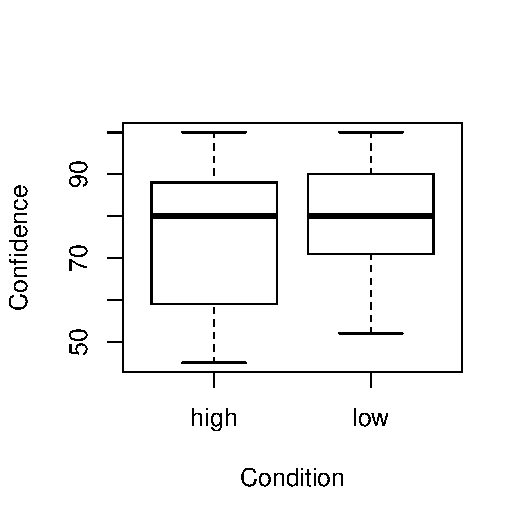
\includegraphics[width=0.5\linewidth,keepaspectratio] {images/groupConfChallengesBoxplot-1}
  \caption{Confidence in group to meet technical challenges, by condition}
  \label{fig:groupConfChallengesBoxplot}
\end{figure}

\begin{figure}
  \centering
   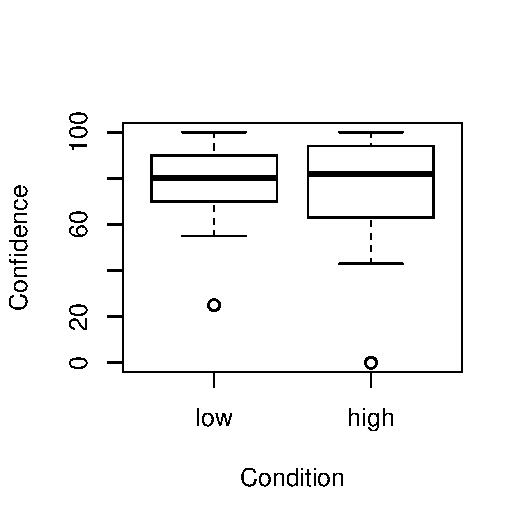
\includegraphics[width=0.5\linewidth,keepaspectratio] {images/indConfChallengesBoxplot-1}
  \caption{Confidence in individual ability to meet technical challenges, by condition}
  \label{fig:indConfChallengesBoxplot}
\end{figure}


\begin{figure}
  \centering
  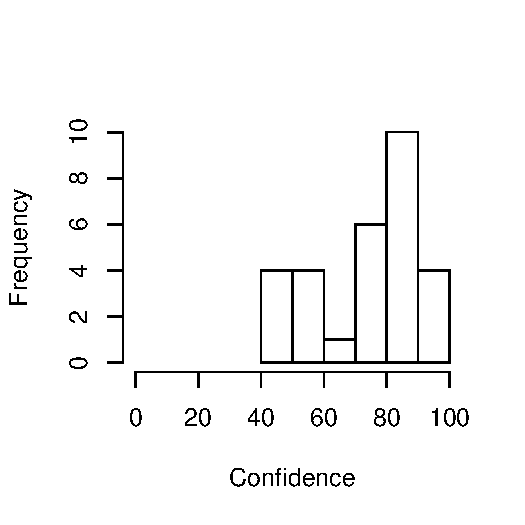
\includegraphics[width=0.5\linewidth,keepaspectratio] {images/histHighGroupConfidence-1}
  \caption{Confidence in group to meet technical challenges (high difficulty condition)}
  \label{fig:groupConfChallengesBoxplot}
\end{figure}

\begin{figure}
  \centering
  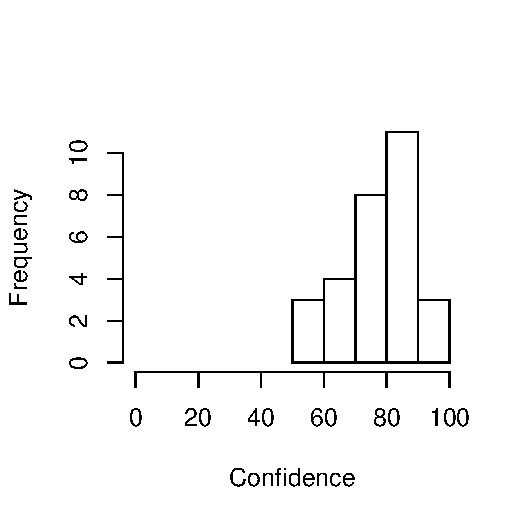
\includegraphics[width=0.5\linewidth,keepaspectratio] {images/histLowGroupConfidence-1}
  \caption{Confidence in group to meet technical challenges (low difficulty condition)}
  \label{fig:histLowGroupConfidence}
\end{figure}

\begin{figure}
  \centering
  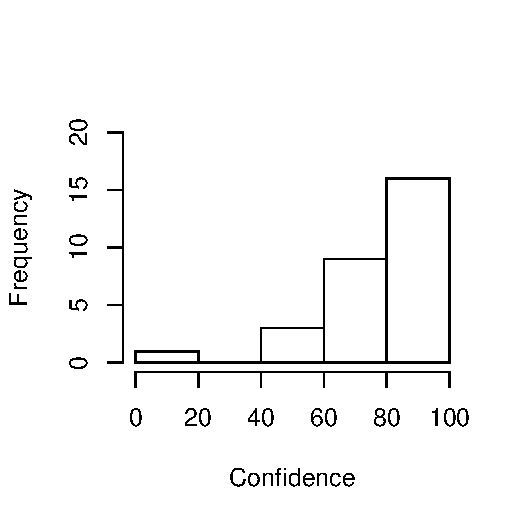
\includegraphics[width=0.5\linewidth,keepaspectratio] {images/histHighIndConfidence-1}
  \caption{Confidence in individual ability to meet technical challenges (high difficulty condition)",}
  \label{fig:histHighIndConfidence}
\end{figure}

\begin{figure}
  \centering
  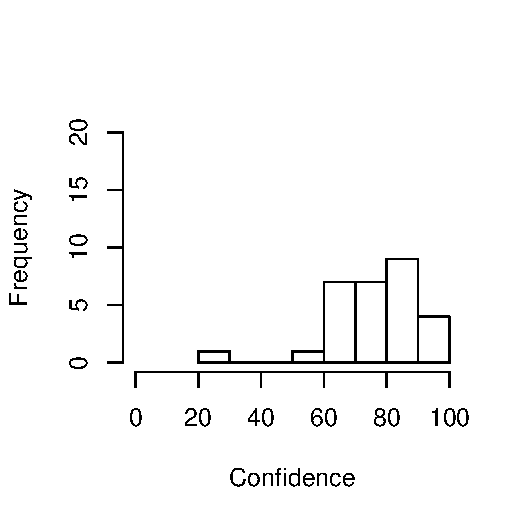
\includegraphics[width=0.5\linewidth,keepaspectratio] {images/histLowIndConfidence-1}
  \caption{Confidence in individual ability to meet technical challenges (high difficulty condition)}
  \label{fig:histLowIndConfidence}
\end{figure}

\begin{figure}
  \centering
  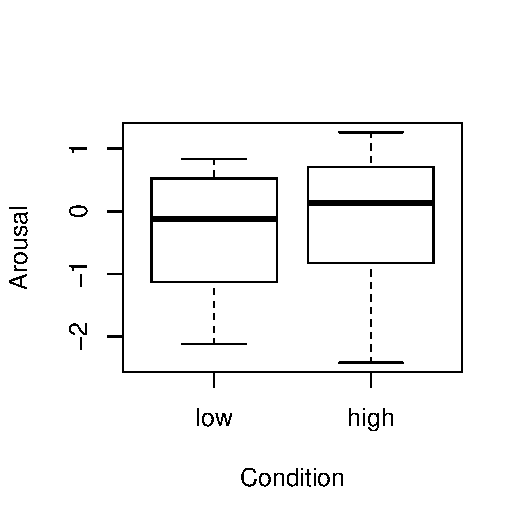
\includegraphics[width=0.5\linewidth,keepaspectratio] {images/arousalFactorPreBoxPlot-1}
  \caption{Athlete arousal prior to experiment, by condition}
        \label{fig:arousalFactorPreBoxPlot}
    \end{figure}

\begin{figure}
  \centering
      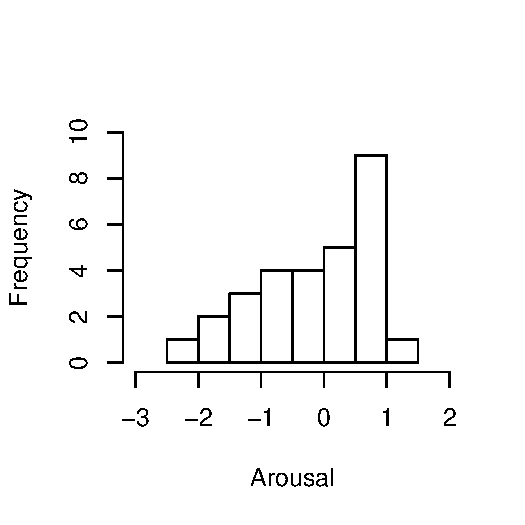
\includegraphics[width=0.5\linewidth,keepaspectratio] {images/histArousalFactorPreHigh-1}
      \caption{Histogram of athlete arousal prior to experiment (high difficulty condition)}
        \label{fig:histArousalFactorPreHigh}
    \end{figure}

\begin{figure}
  \centering
  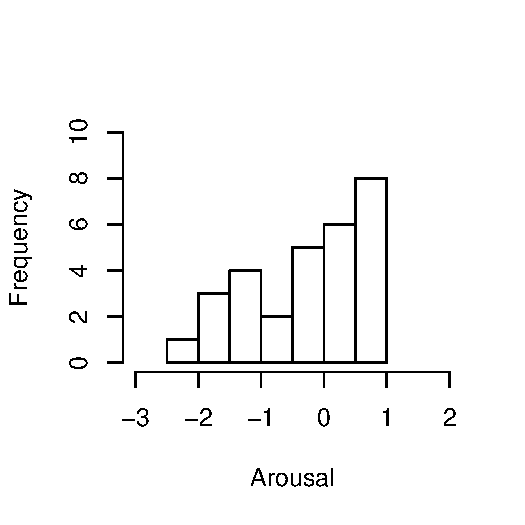
\includegraphics[width=0.5\linewidth,keepaspectratio] {images/histArousalFactorPreLow-1}
      \caption{Histogram of athlete arousal prior to experiment (low difficulty condition)}
  \caption{title}
    \label{fig:histArousalFactorPreLow}
\end{figure}












\subsection{Analysis of Study Predictions\label{app6:analysisStudyPredictions}}





\subsubsection{Analysis of Post-Experiment data\label{app6:postExperimentData}}


\myparagraph{Differences by condition\label{app6:conditionDifferences}}

\begin{figure}
    \centering
    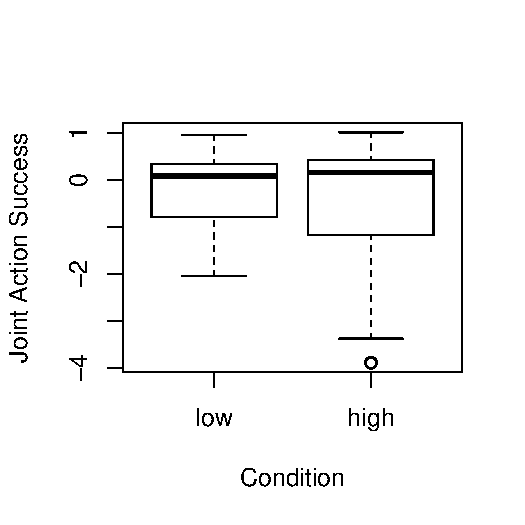
\includegraphics[width=0.5\linewidth,keepaspectratio] {images/groupJointActionSuccessPostBoxPlot-1}
    \caption{Athlete post-experiment perceptions of joint action success by condition}
              \label{fig:groupJointActionSuccessPostBoxPlot}
\end{figure}

\begin{figure}
  \centering
  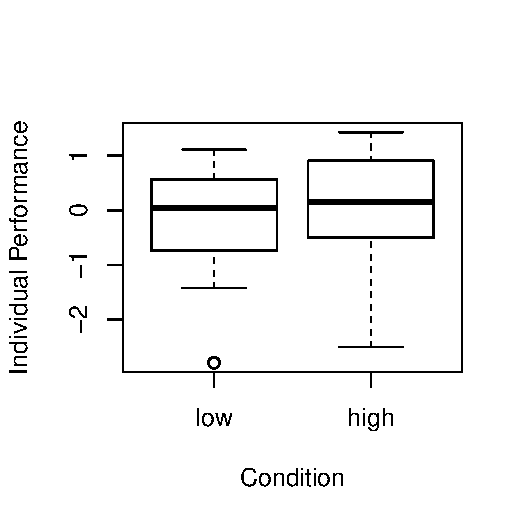
\includegraphics[width=0.5\linewidth,keepaspectratio] {images/indComponentPerformancePostBoxPlot-1}
  \caption{Athlete post-experiment perceptions of individual performance by condition}
    \label{fig:indComponentPerformancePostBoxPlot}
\end{figure}

\begin{figure}
  \centering
  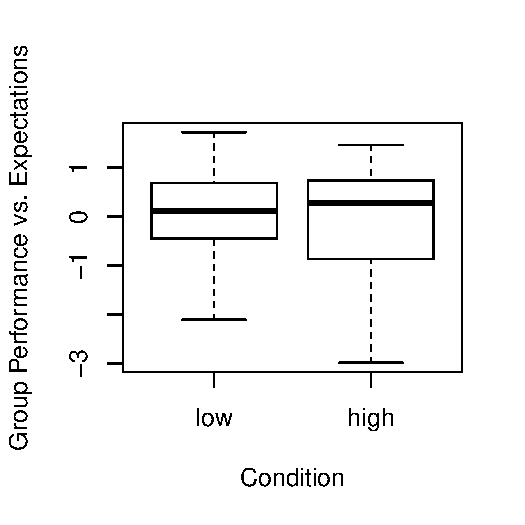
\includegraphics[width=0.5\linewidth,keepaspectratio] {images/groupPerfExpPostBoxPlot-1}
          \label{fig:groupPerfExpPostBoxPlot}
        \caption{Athlete post-experiment perceptions of group performance relative to expectations by condition}
\end{figure}


\begin{figure}
  \centering
      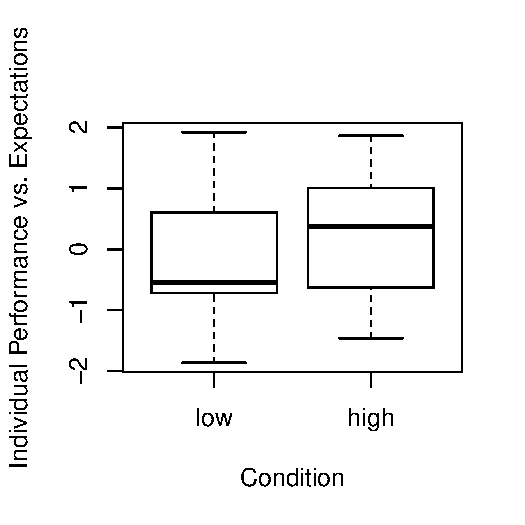
\includegraphics[width=0.5\linewidth,keepaspectratio] {images/indPerfExpPostBoxPlot-1}
              \label{fig:indPerfExpPostBoxPlot}
              \caption{Athlete post-experiment perceptions of individual performance relative to expectations by condition}
\end{figure}






\myparagraph{Model Structure\label{app6:modelStructure}}



\myparagraph{ICC Values\label{app6:postExperimentICC}}

% latex table generated in R 3.3.0 by xtable 1.8-2 package
% Mon Oct 16 19:11:18 2017
\begin{table}[ht]
\centering
\begin{tabular}{rrcccc}
  \hline
 & variable & session & sex & team & location \\ 
  \hline
1 & PerformExpected & 0.06 & 0.06 & 0.08 & 0.01 \\ 
  2 & GroupClick & 0.14 & -0.03 & 0.09 & 0.08 \\ 
  3 & GroupBonding & 0.21 & -0.01 & 0.24 & 0.15 \\ 
   \hline
\end{tabular}
\caption{Intra class correlations of variables of interest according to groups} 
\label{tab:ICCTable}
\end{table}


% latex table generated in R 3.3.0 by xtable 1.8-2 package
% Mon Oct 16 21:13:43 2017
\begin{table}[ht]
\centering
\begin{tabular}{rlrr}
  \hline
 & Session & Mean & SD \\ 
  \hline
1 & ShandongWomenHigh & 2.56 & 1.36 \\ 
  2 & ShandongMenHigh & 2.38 & 1.36 \\ 
  3 & BeijingWomenHigh & 2.81 & 1.38 \\ 
  4 & BeijingMenHigh & 2.72 & 1.23 \\ 
  5 & ShandongWomenLow & 2.75 & 1.34 \\ 
  6 & ShandongMenLow & 3.19 & 1.33 \\ 
  7 & BeijingWomenLow & 1.62 & 1.15 \\ 
  8 & BeijingMenLow & 1.94 & 1.12 \\ 
   \hline
\end{tabular}
\caption{Mean and standard deviation of performance outcome according to experiment session} 
\label{tab:outcomeAvgSdSession}
\end{table}



ICC values for perceptions of group performance relative to prior expectations were very low for each grouping variables (all $r's < .10$), indicating that between-group variance in perceptions of group performance was minimal across categories of experiment session, sex, team, and experiment location (Beijing or Shandong).  ICC values for group click were also low, with the exception being the value for experimental session ($r = .14$).  ICC values for social bonding to the training group did show some evidence of moderate between-group variance, by team ($r = .24$) and by experiment session ($r = .21$).







\myparagraph{Model Assumptions\label{app6:postExperimentModelAssumptions}}

%%Model 1
\begin{figure}[htbp]
    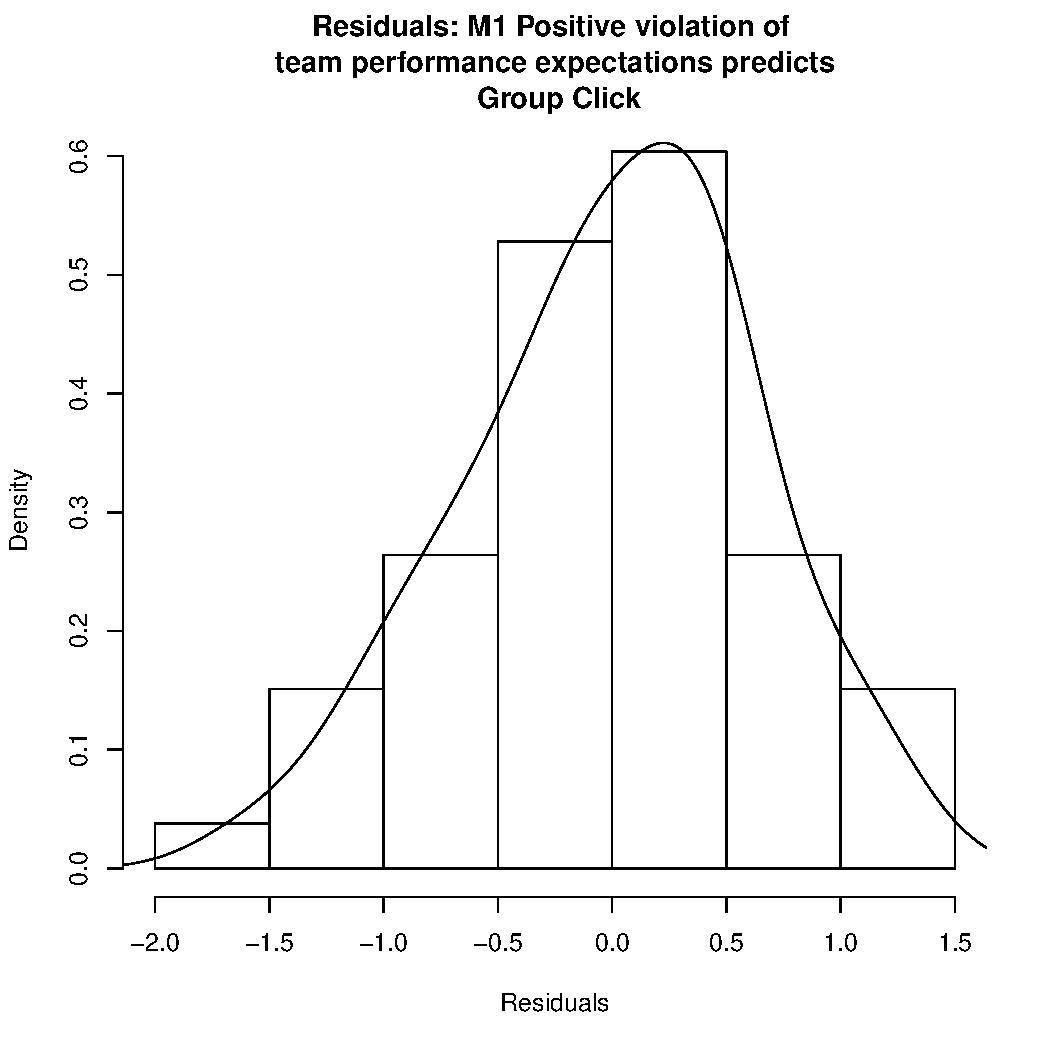
\includegraphics[scale =.4]{images/TEM1Hist.pdf}
    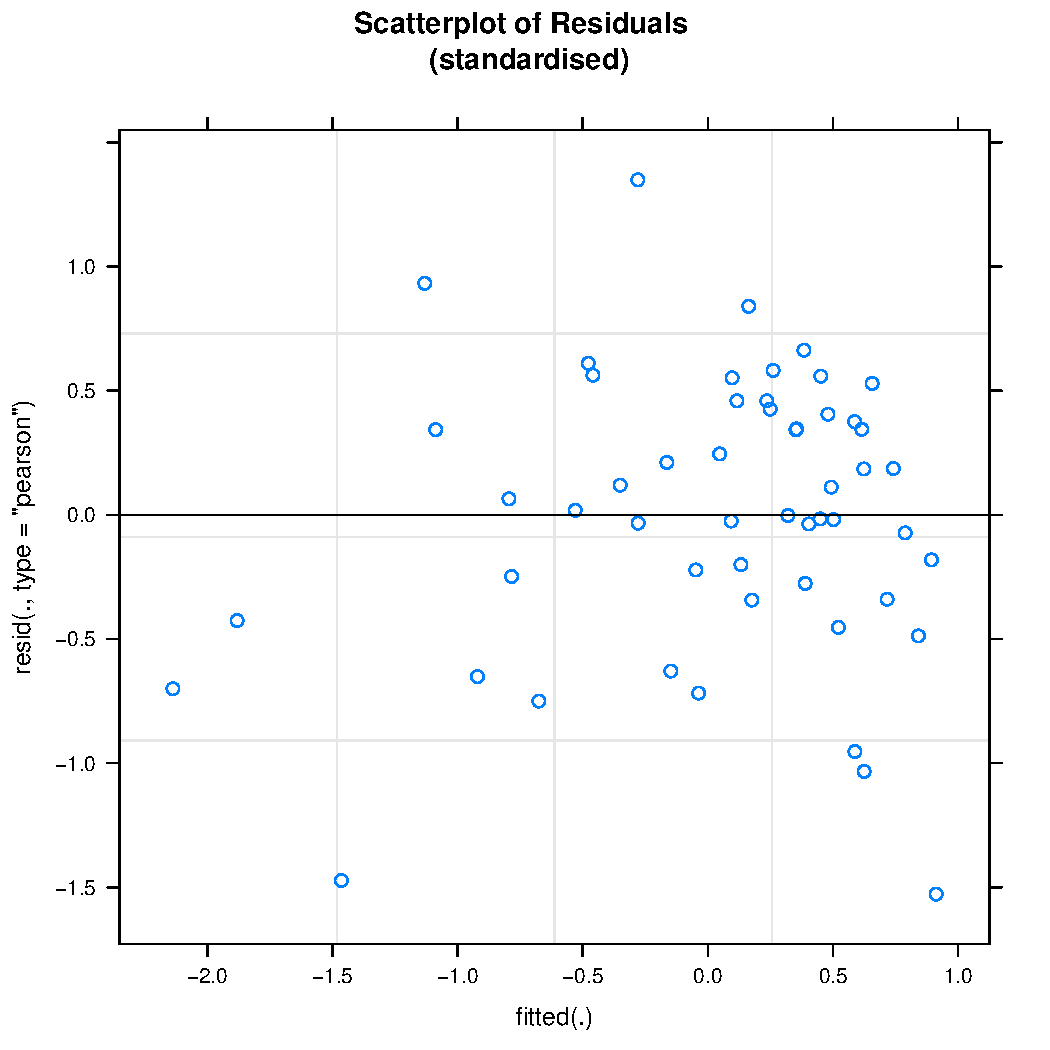
\includegraphics[scale =.4]{images/TEM1Scatter.pdf}
    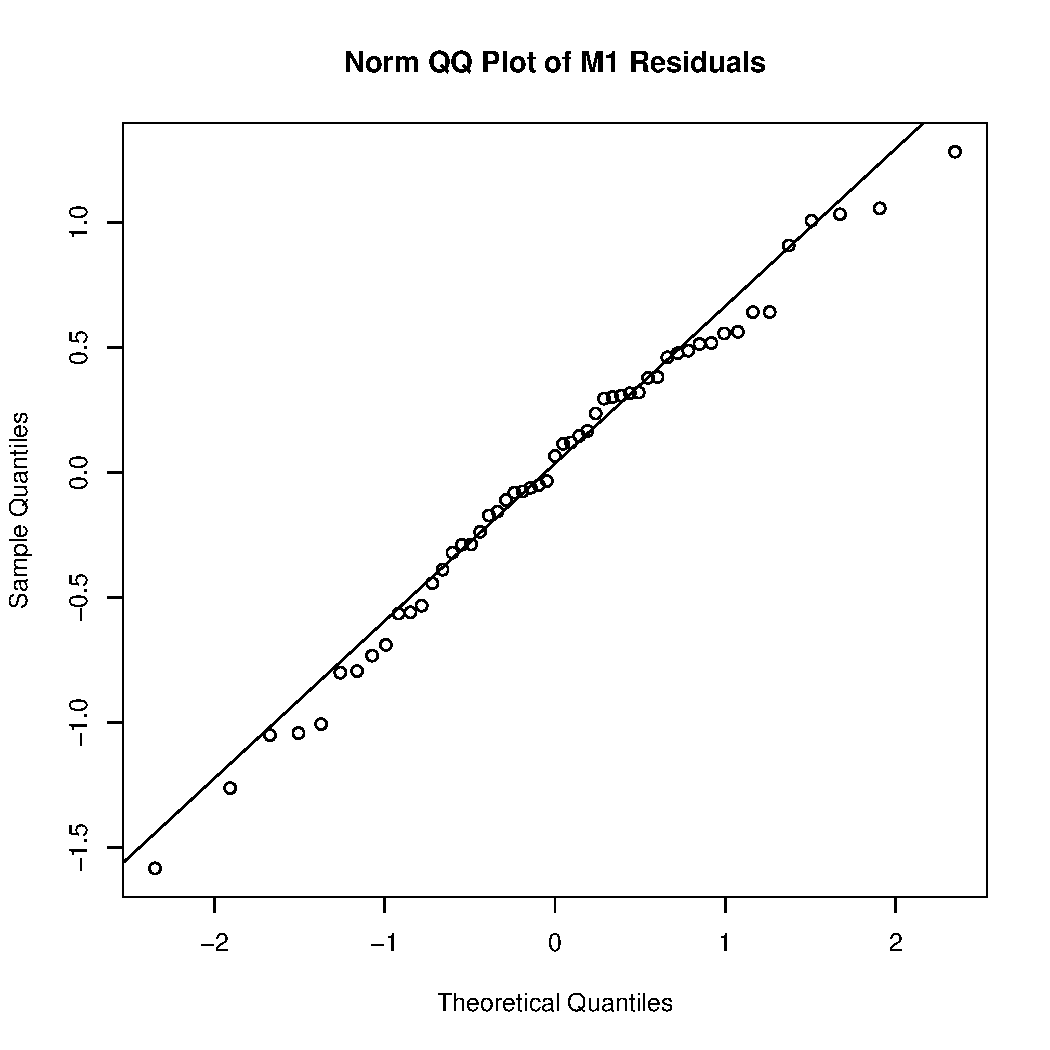
\includegraphics[scale =.4]{images/TEM1QQNorm.pdf}
    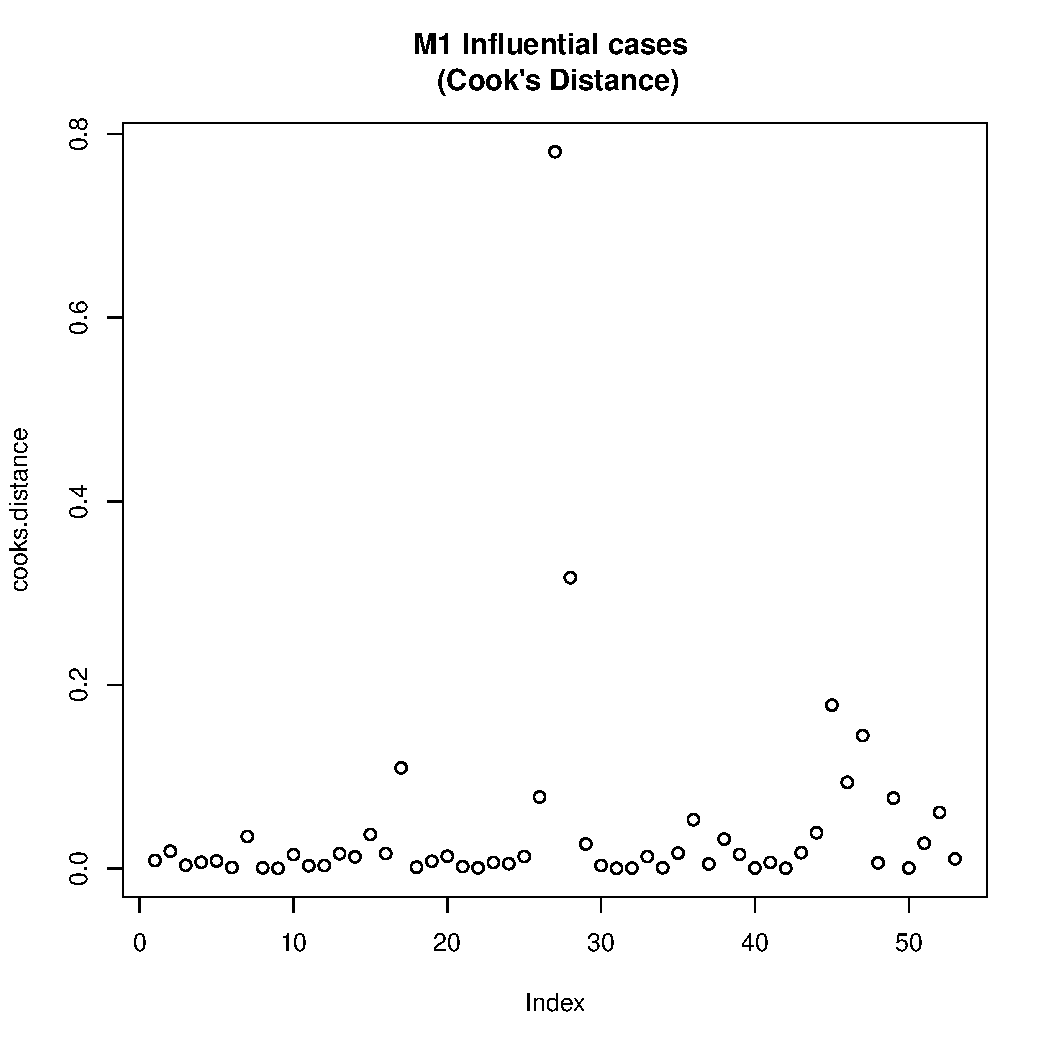
\includegraphics[scale =.4]{images/TEM1CooksD.pdf}
    \caption{Model 1 Assumptions: Positive violation of group performance expectations predicts feelings of Team Click, moderated by condition}
    \label{fig:M1Assumptions}
\end{figure}

%%Model 1a
\begin{figure}[htbp]
    \includegraphics[scale =.4]{images/TEM1aHist.pdf}
    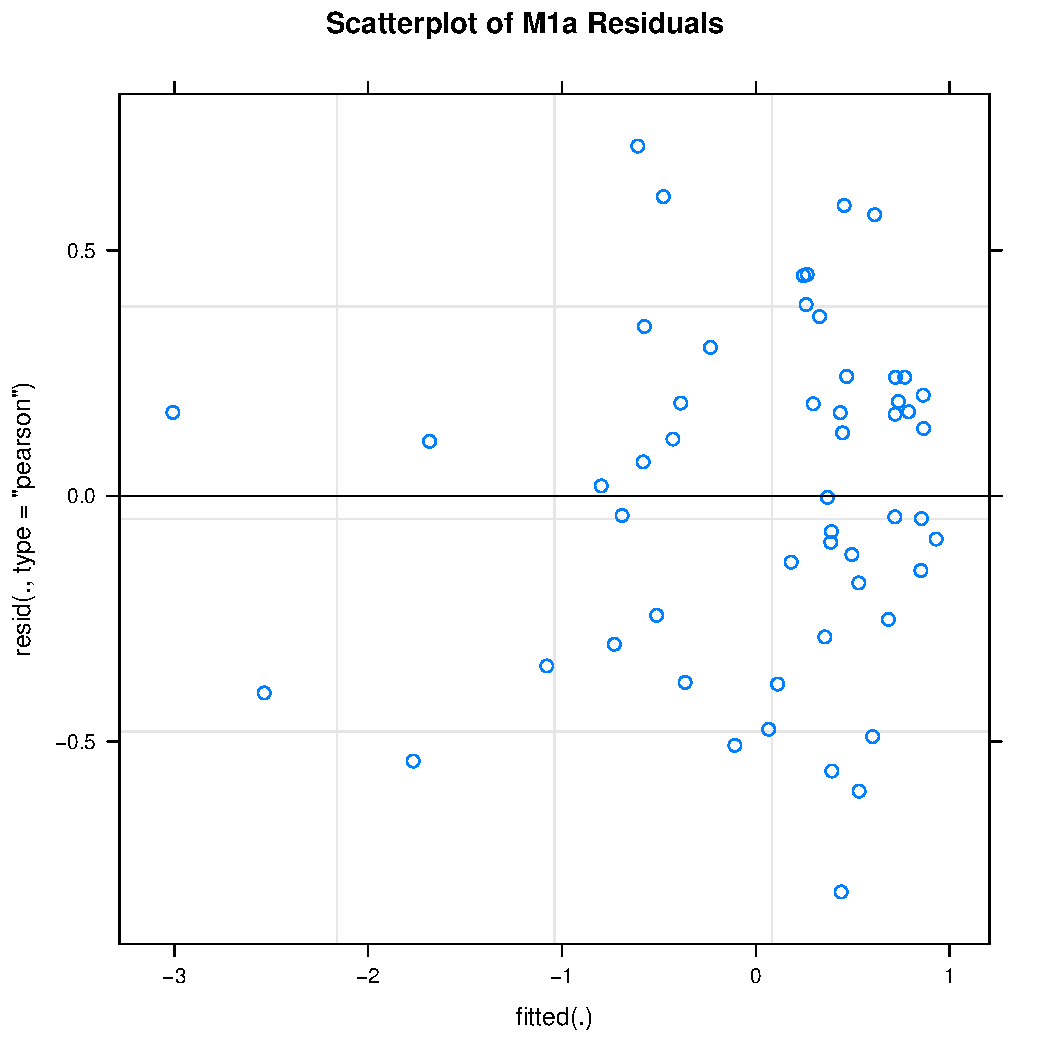
\includegraphics[scale =.4]{images/TEM1aScatter.pdf}
    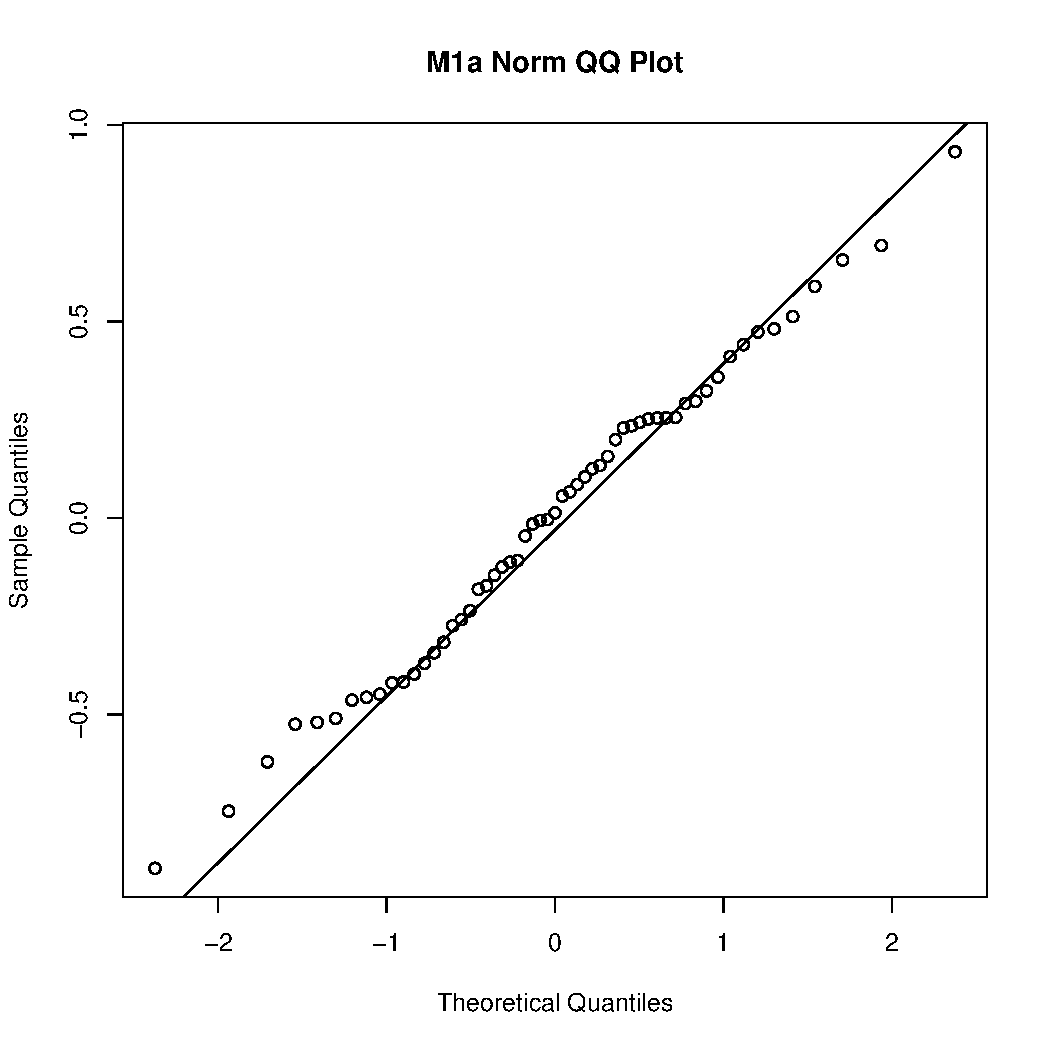
\includegraphics[scale =.4]{images/TEM1aQQNorm.pdf}
    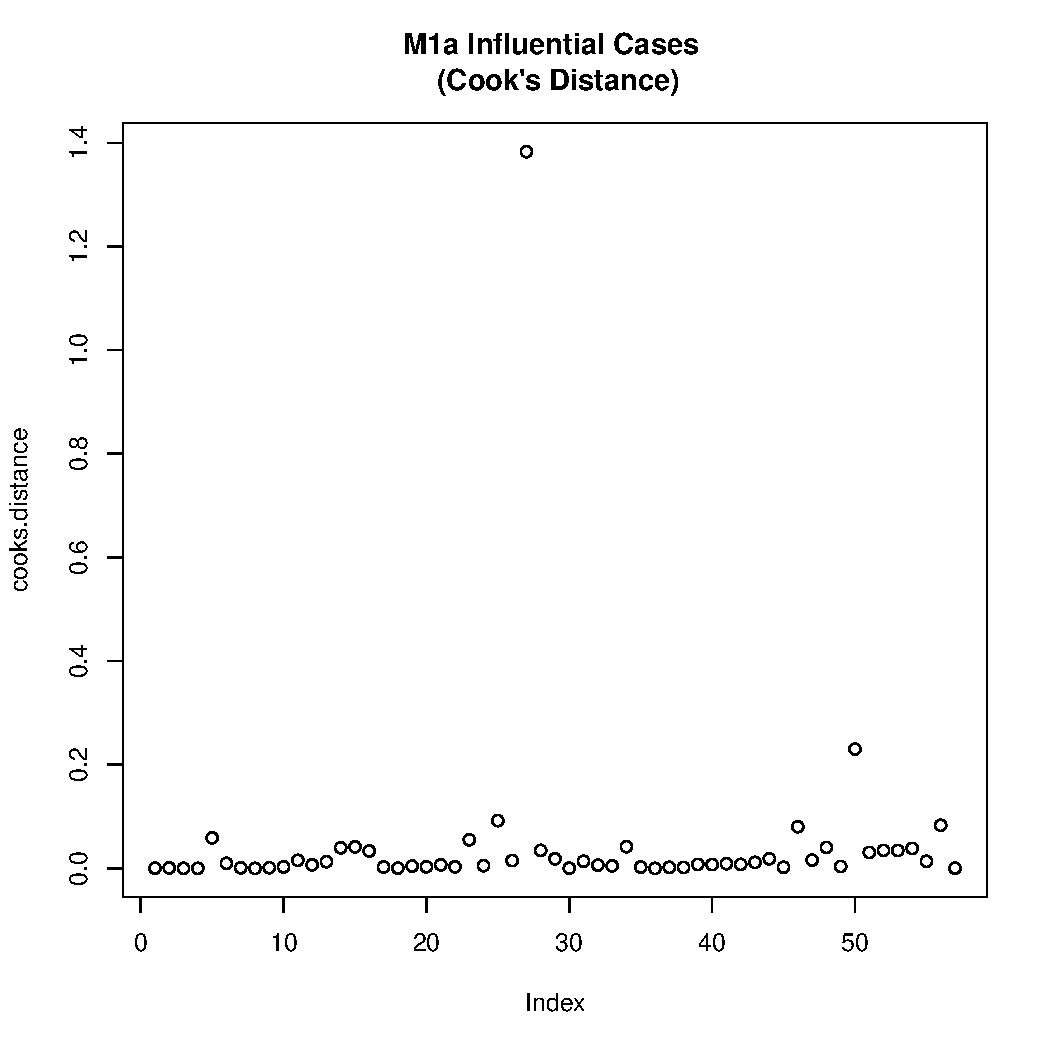
\includegraphics[scale =.4]{images/TEM1aCooksD.pdf}
    \caption{Model 1a Assumptions: The interaction between positive violation of group performance expectations and perceptions of joint action success predicts feelings of Team Click}
    \label{fig:M1aAssumptions}
\end{figure}


%%Model 2
\begin{figure}[htbp]
    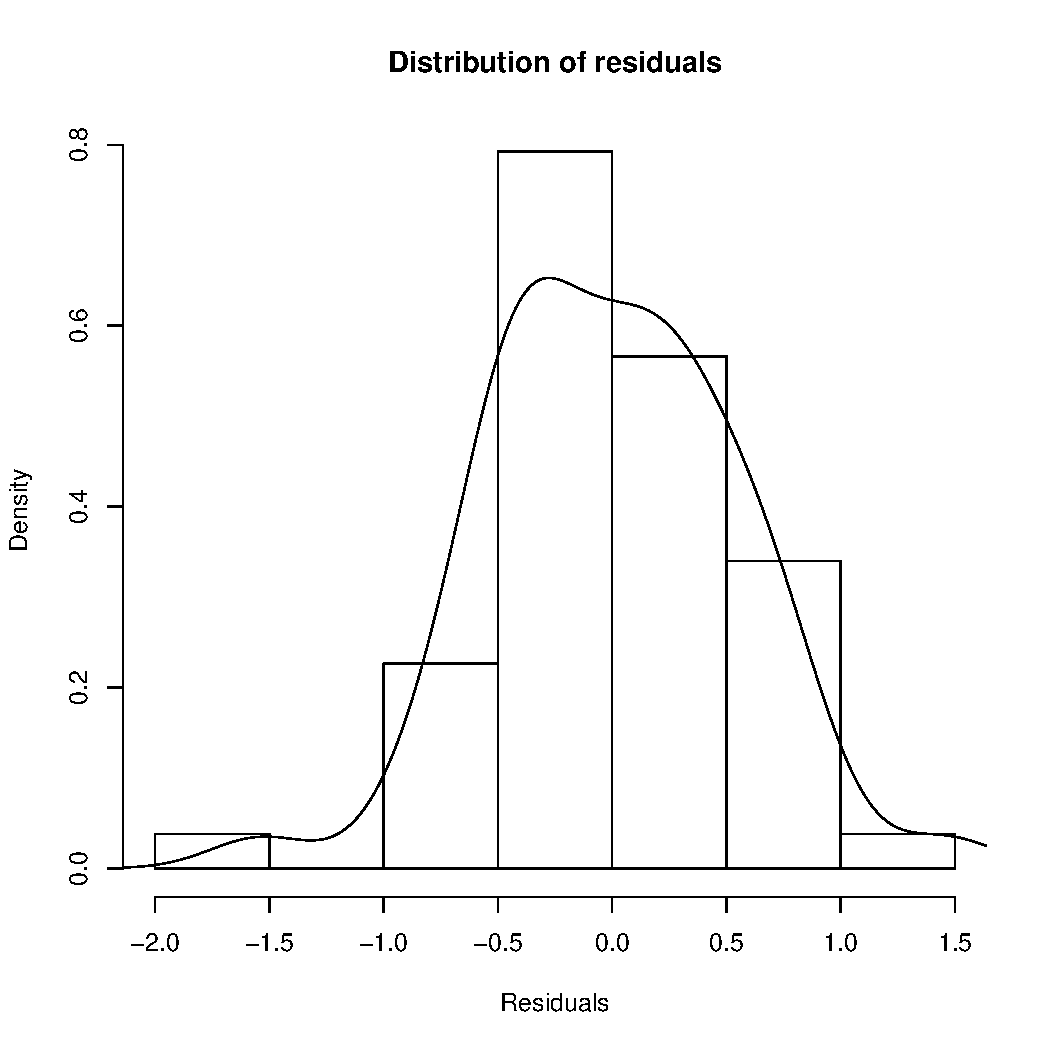
\includegraphics[scale =.4]{images/TEM2Hist.pdf}
    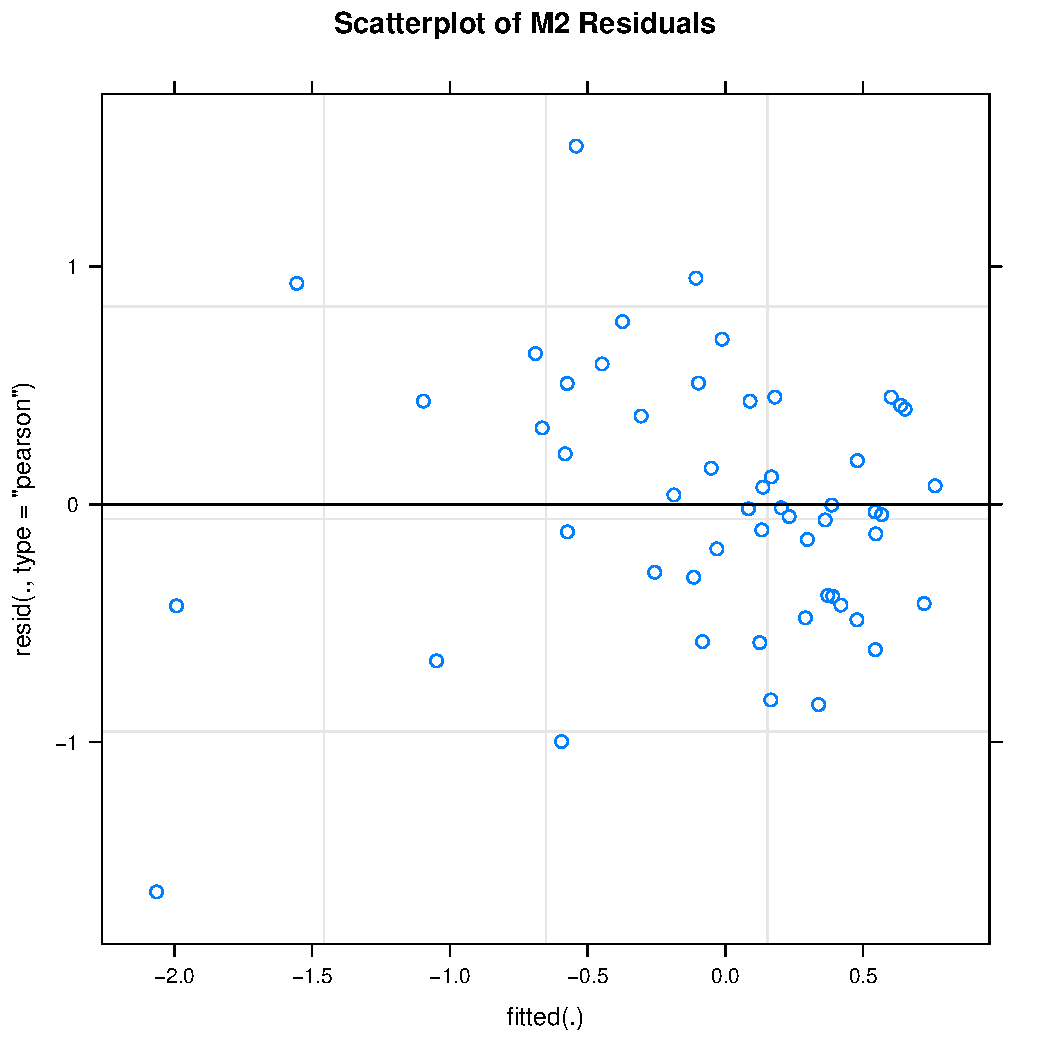
\includegraphics[scale =.4]{images/TEM2Scatter.pdf}
    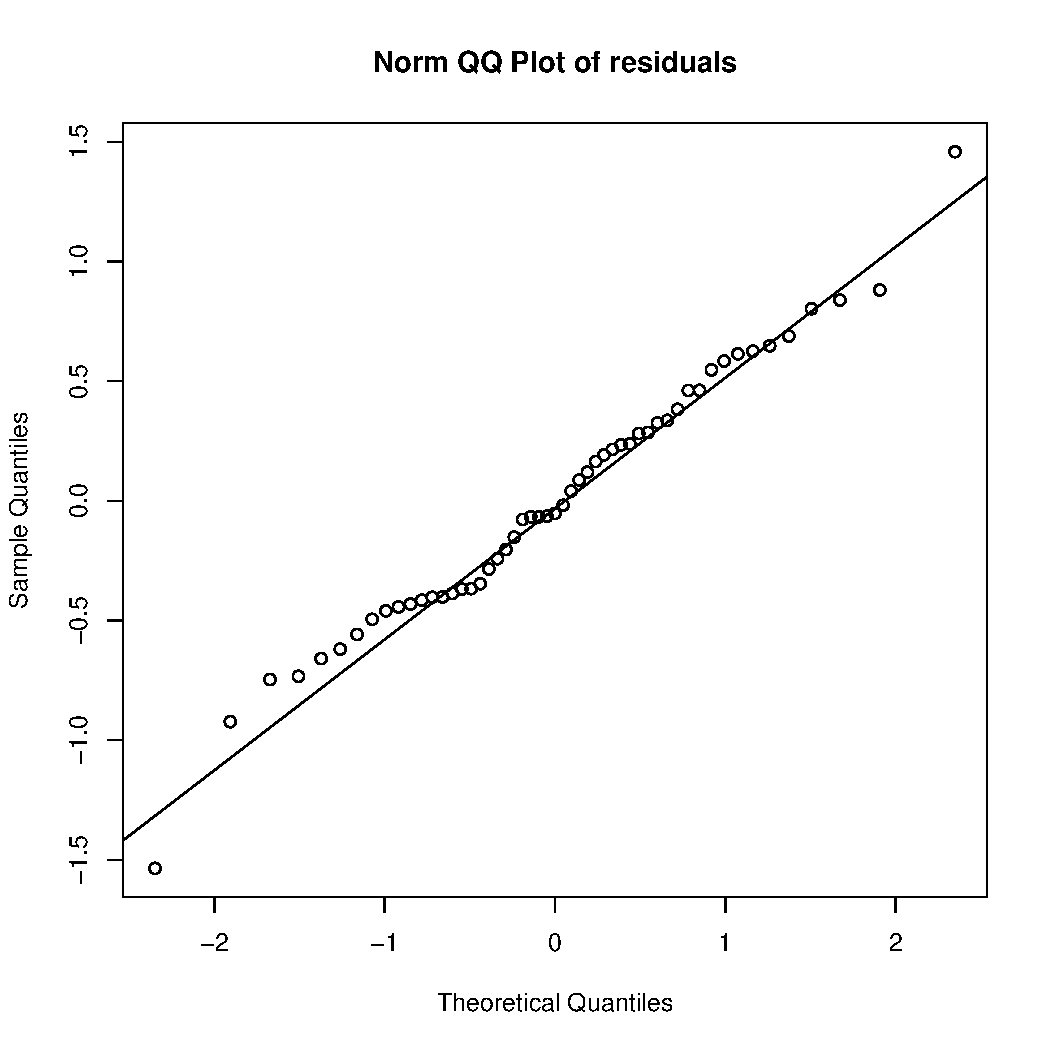
\includegraphics[scale =.4]{images/TEM2QQNorm.pdf}
    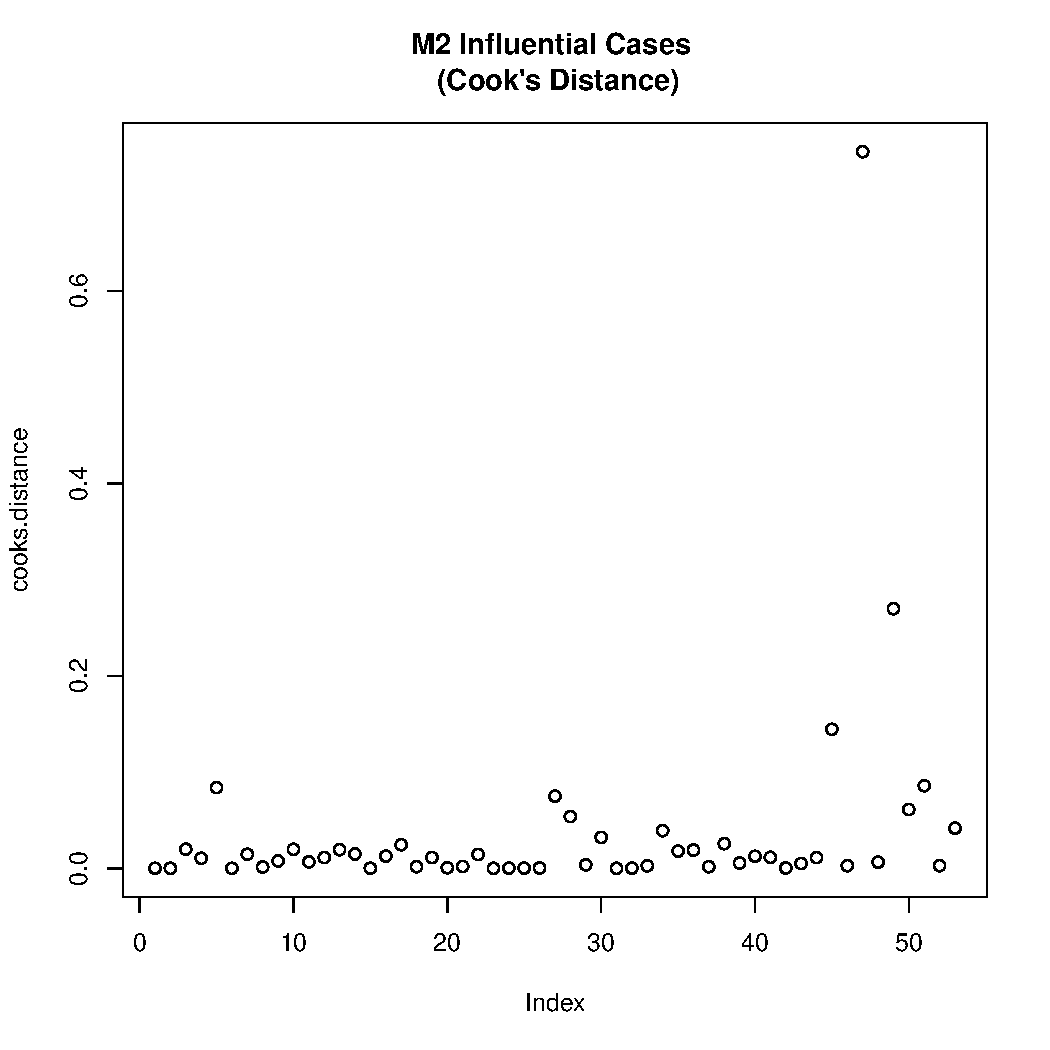
\includegraphics[scale =.4]{images/TEM2CooksD.pdf}
    \caption{Model 2 Assumptions: Feelings of Team Click predict feelings of Social Bonding}
    \label{fig:M2Assumptions}
\end{figure}


%%Model 3
\begin{figure}[htbp]
    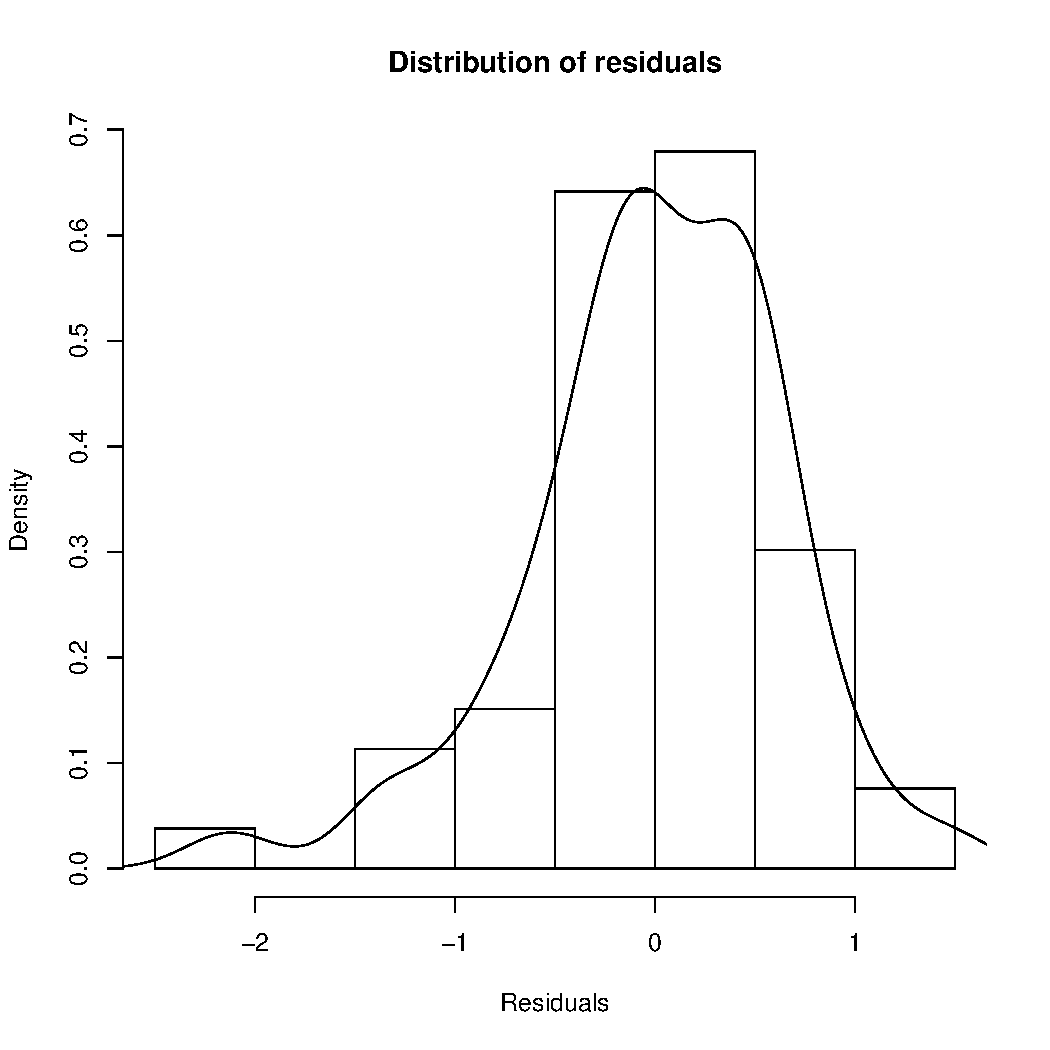
\includegraphics[scale =.4]{images/TEM3Hist.pdf}
    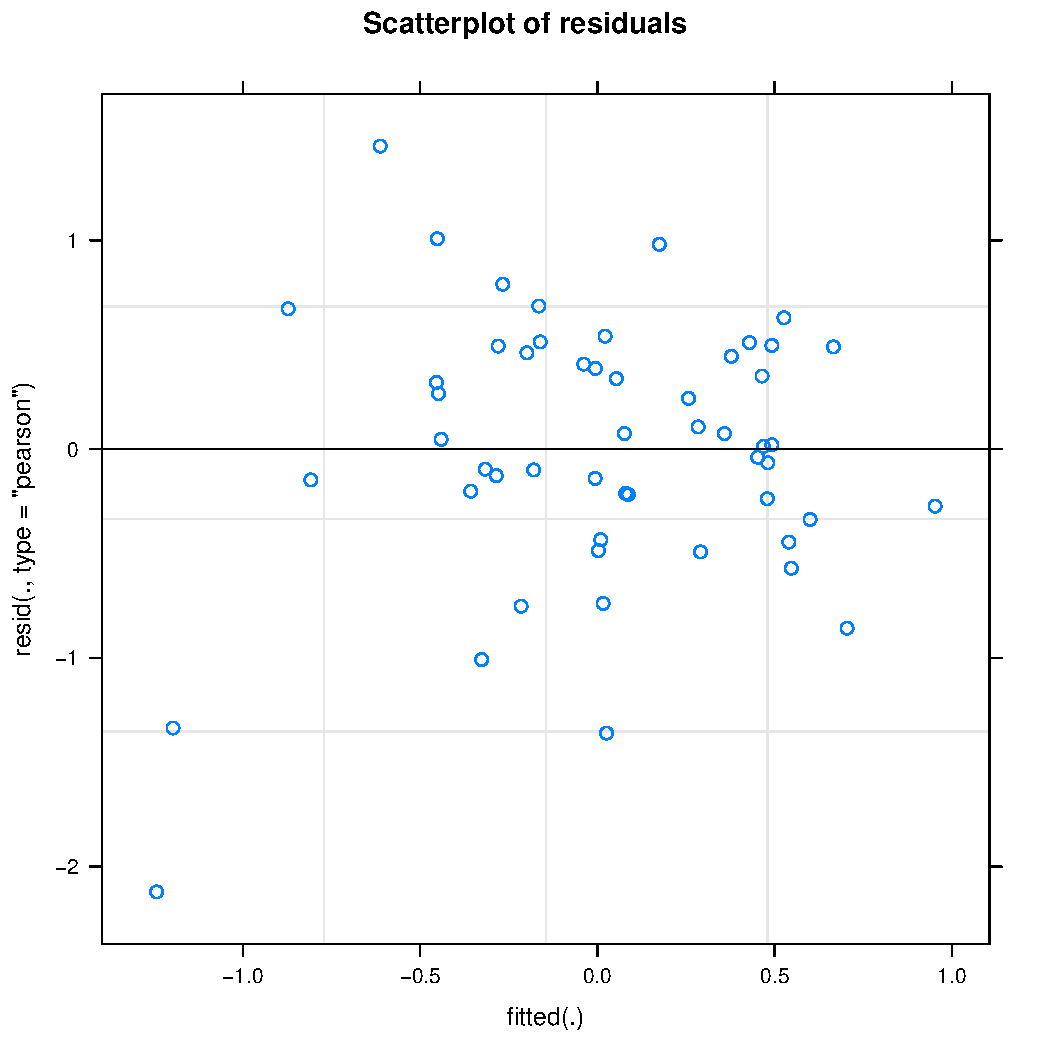
\includegraphics[scale =.4]{images/TEM3Scatter.pdf}
    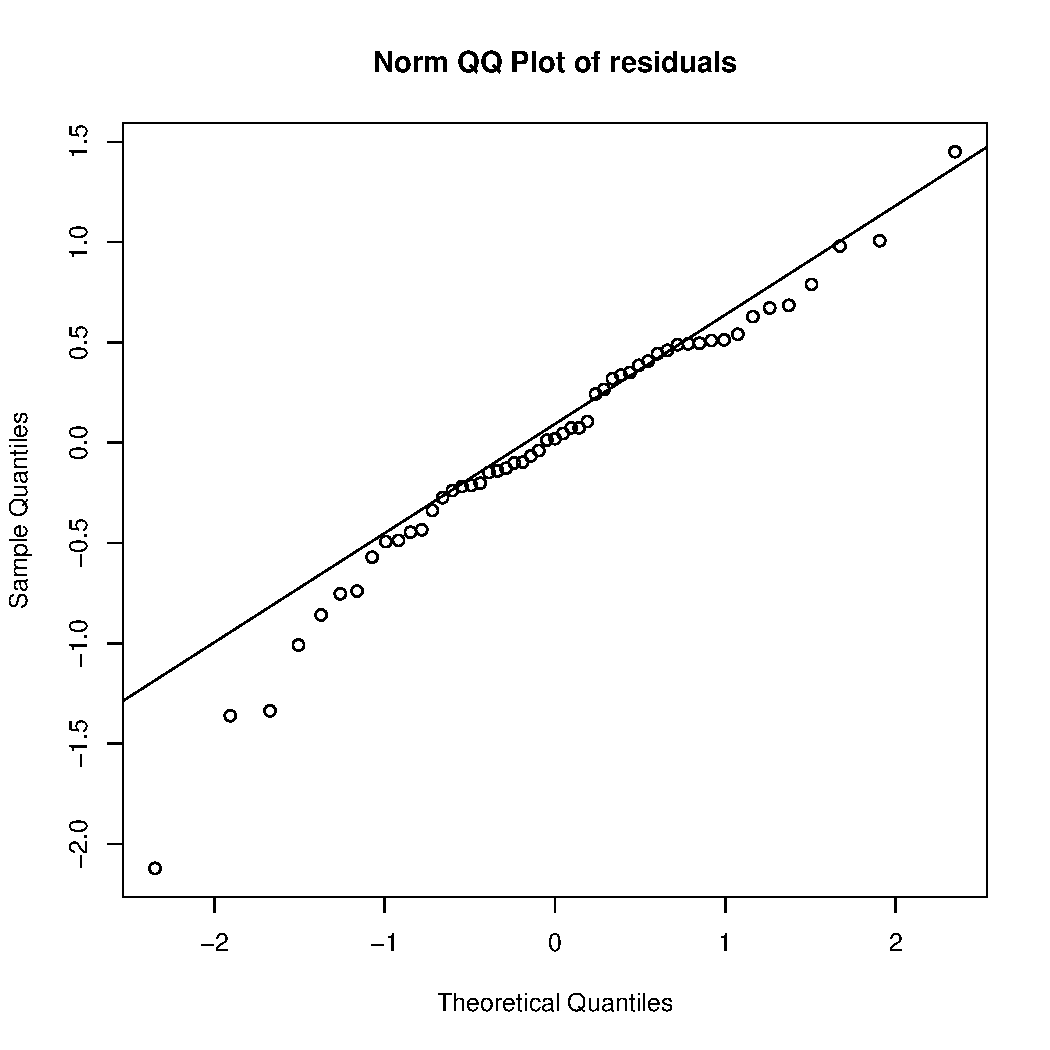
\includegraphics[scale =.4]{images/TEM3QQNorm.pdf}
    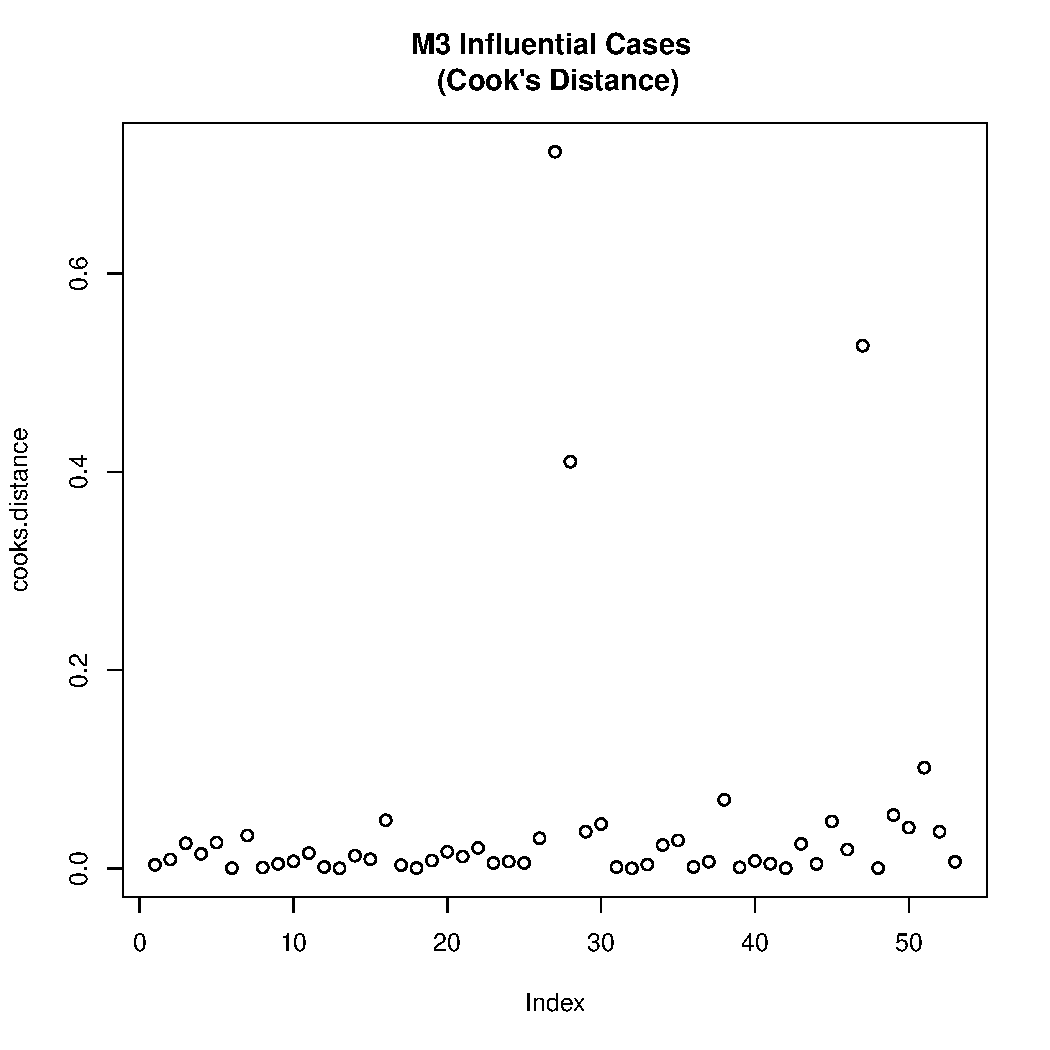
\includegraphics[scale =.4]{images/TEM3CooksD.pdf}
    \caption{Model 3 Assumptions: Positive violation of group performance expectations predicts feelings of Social Bonding, moderated by condition}
    \label{fig:M3Assumptions}
\end{figure}





\subsection{Analysis of Pre-post Experiment Survey Data}




\myparagraph{Condition Differences\label{app6:conditionDifferencesPrePost}}



\begin{figure}
  \centering
    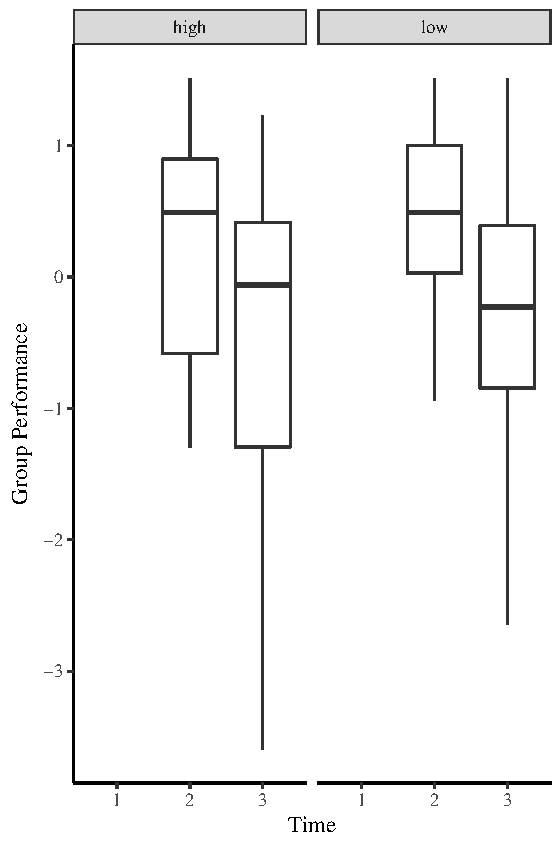
\includegraphics[width=0.5\linewidth,keepaspectratio] {images/groupPerfConfPlot}
    \label{fig:groupPerfConfPlot}
    \caption{Group performance vs expectations by time and condition}
\end{figure}


\begin{figure}
  \centering
  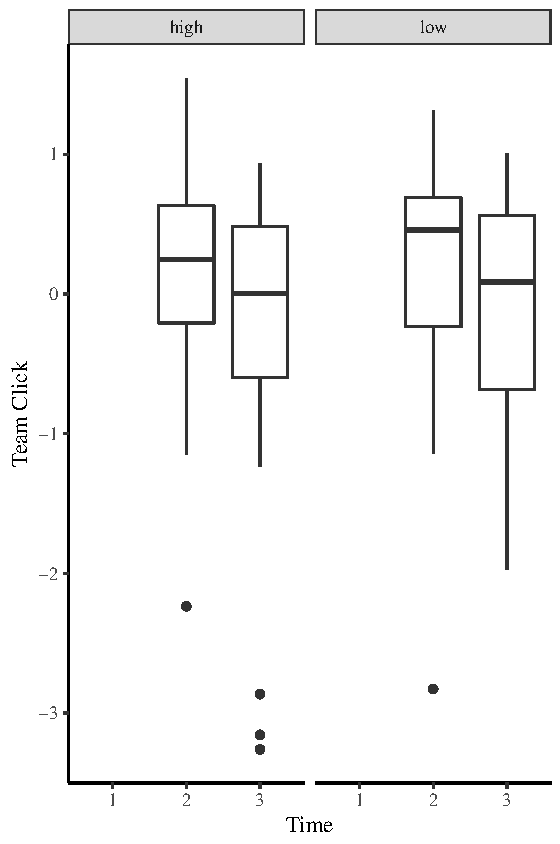
\includegraphics[width=0.5\linewidth,keepaspectratio] {images/prePostClickPLot}
  \label{fig:prePostClickPLot}
  \caption{Group click by time and condition}
\end{figure}

\begin{figure}
  \centering
  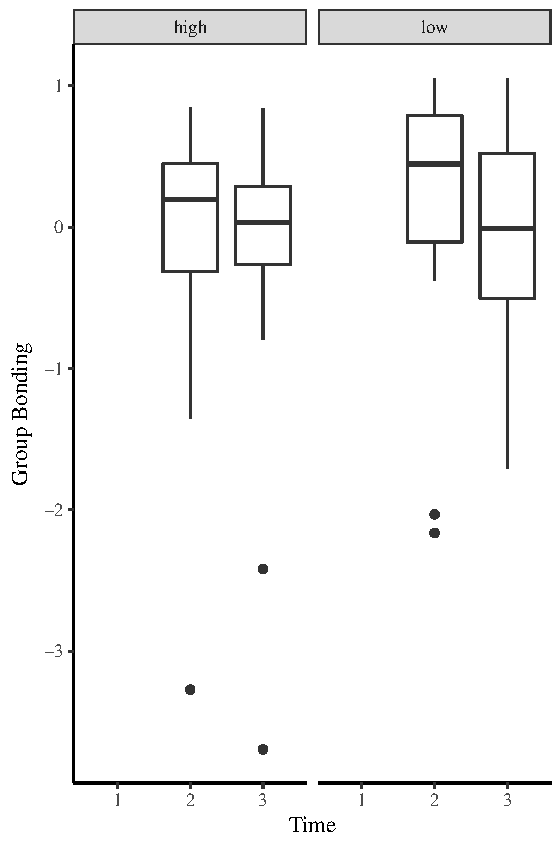
\includegraphics[width=0.5\linewidth,keepaspectratio] {images/prePostBondingPlot}
    \label{fig:prePostBondingPlot}
  \caption{Social bonding by time and condition}
\end{figure}




\myparagraph{Construction of new variables expressing change in variables over time (pre- to post-Experiment)\label{app6:newVariablesPrePostChange}}



\myparagraph{Model Selection \label{app6:modelSelectionPrePost}}

\input{images/ICCtablePrePost.tex}












\subsubsection{Analysis of study predictions}


\myparagraph{Model Assumptions\label{app6:prePostExperimentModelAssumptions}}

%M2.1
\begin{figure}[htbp]
    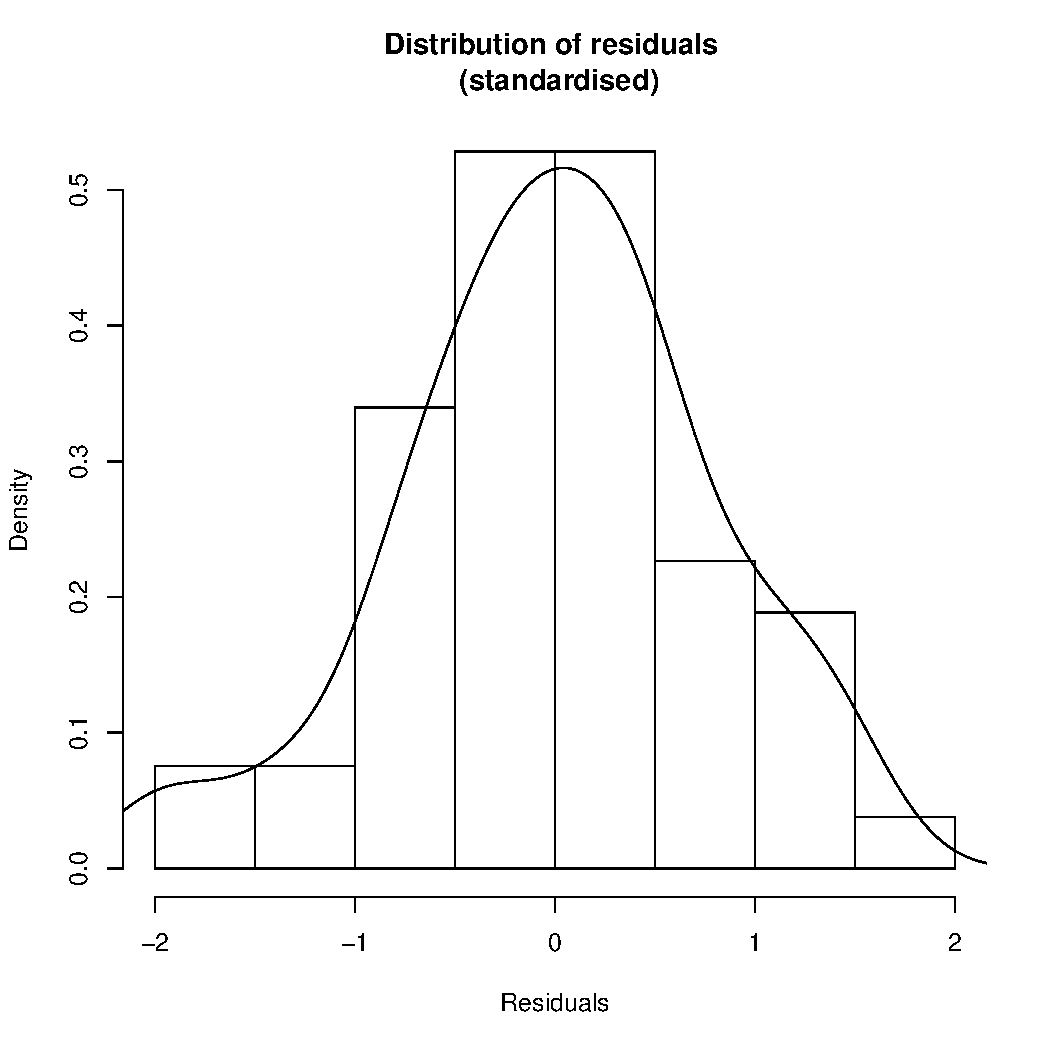
\includegraphics[scale =.4]{images/TEM21Hist.pdf}
    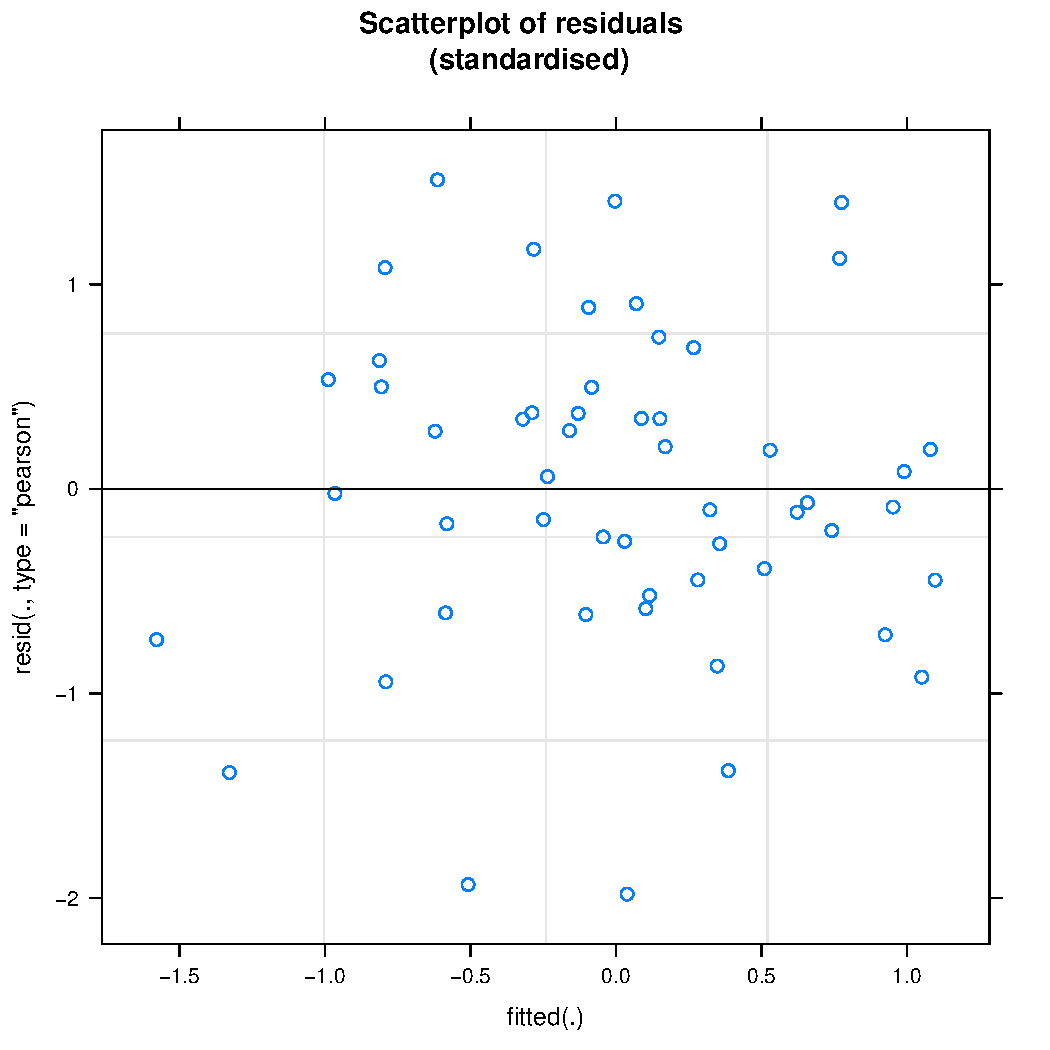
\includegraphics[scale =.4]{images/TEM21Scatter.pdf}
    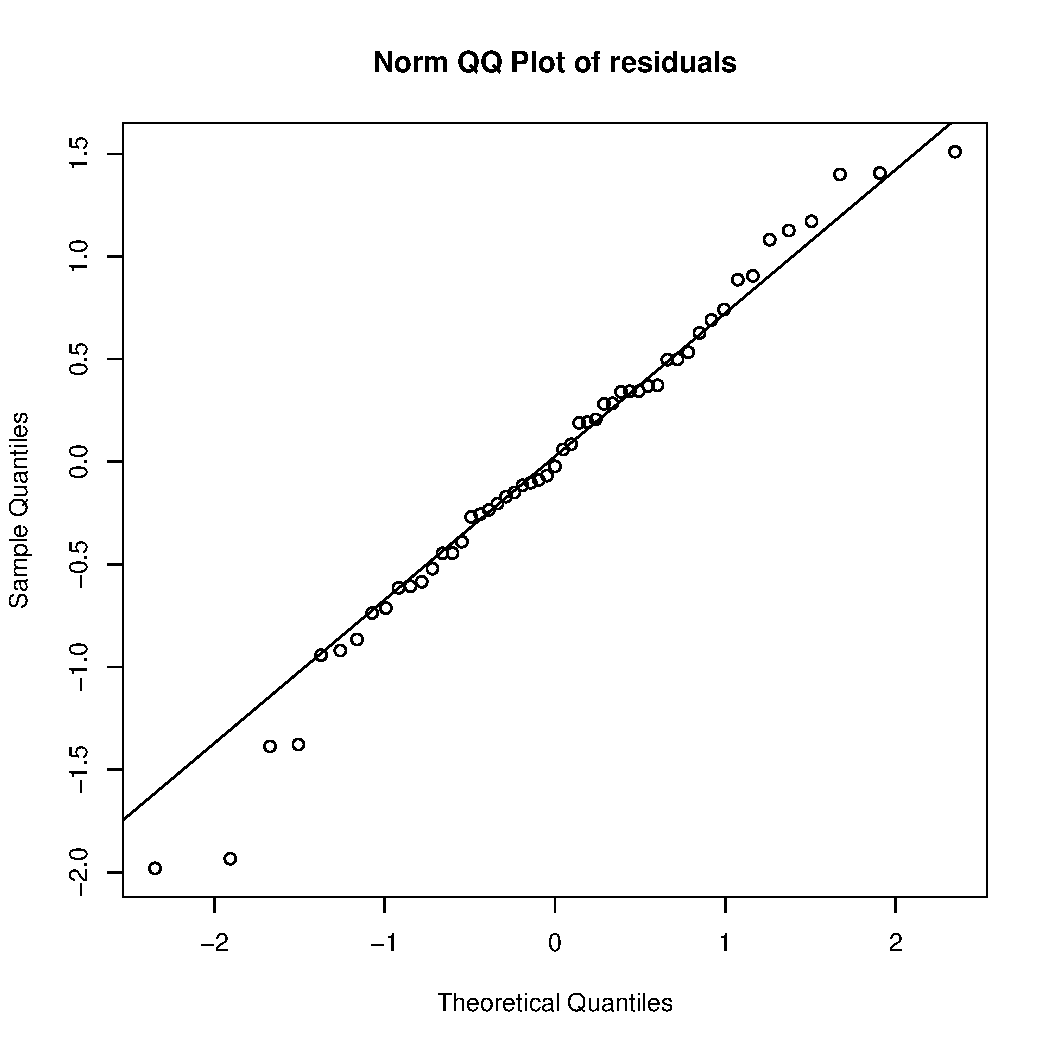
\includegraphics[scale =.4]{images/TEM21QQNorm.pdf}
    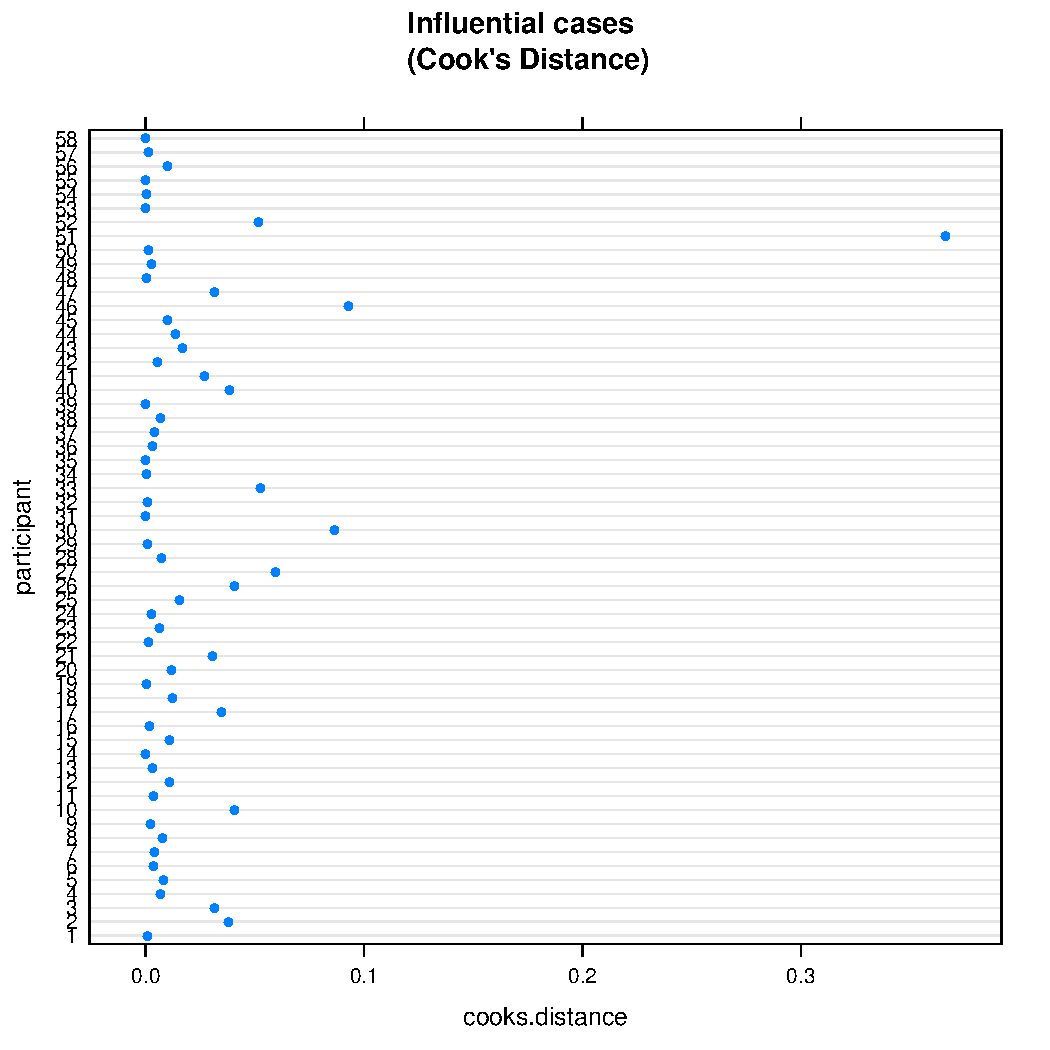
\includegraphics[scale =.4]{images/TEM21CooksD.pdf}
    \caption{Model 2.1 Assumptions: More positive change in perceptions of group performance predicts feelings of Social Bonding, moderated by condition}
    \label{fig:M21Assumptions}
\end{figure}

%M2.2
\begin{figure}[htbp]
    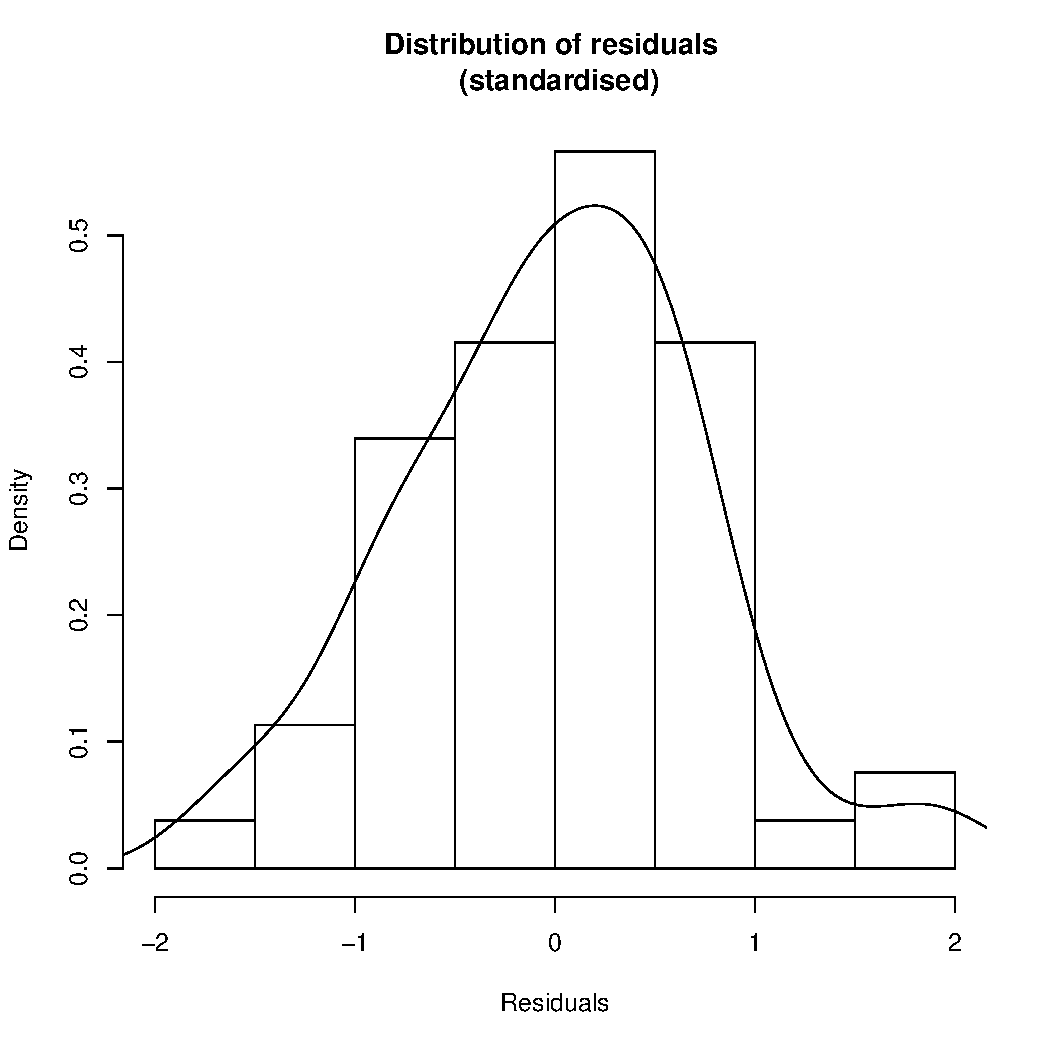
\includegraphics[scale =.4]{images/TEM22Hist.pdf}
    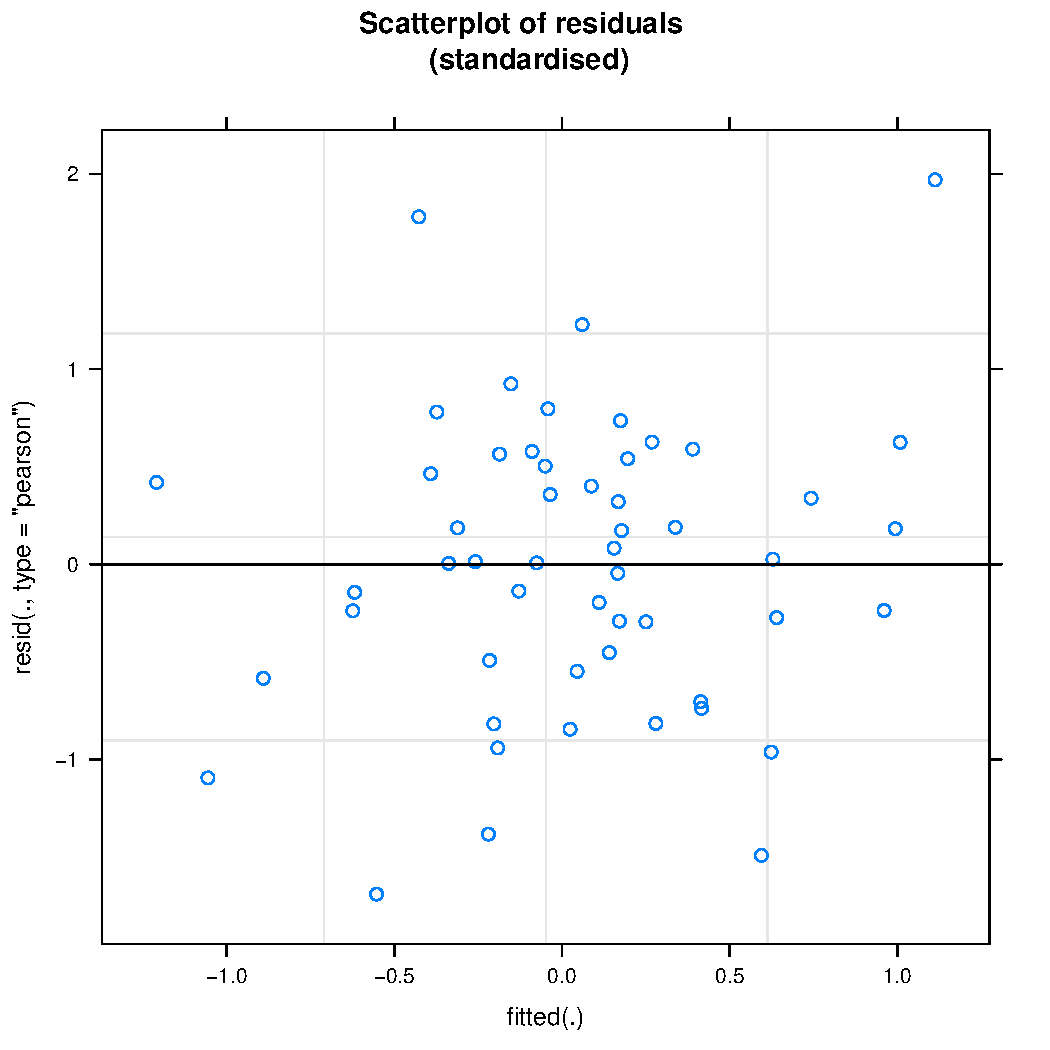
\includegraphics[scale =.4]{images/TEM22Scatter.pdf}
    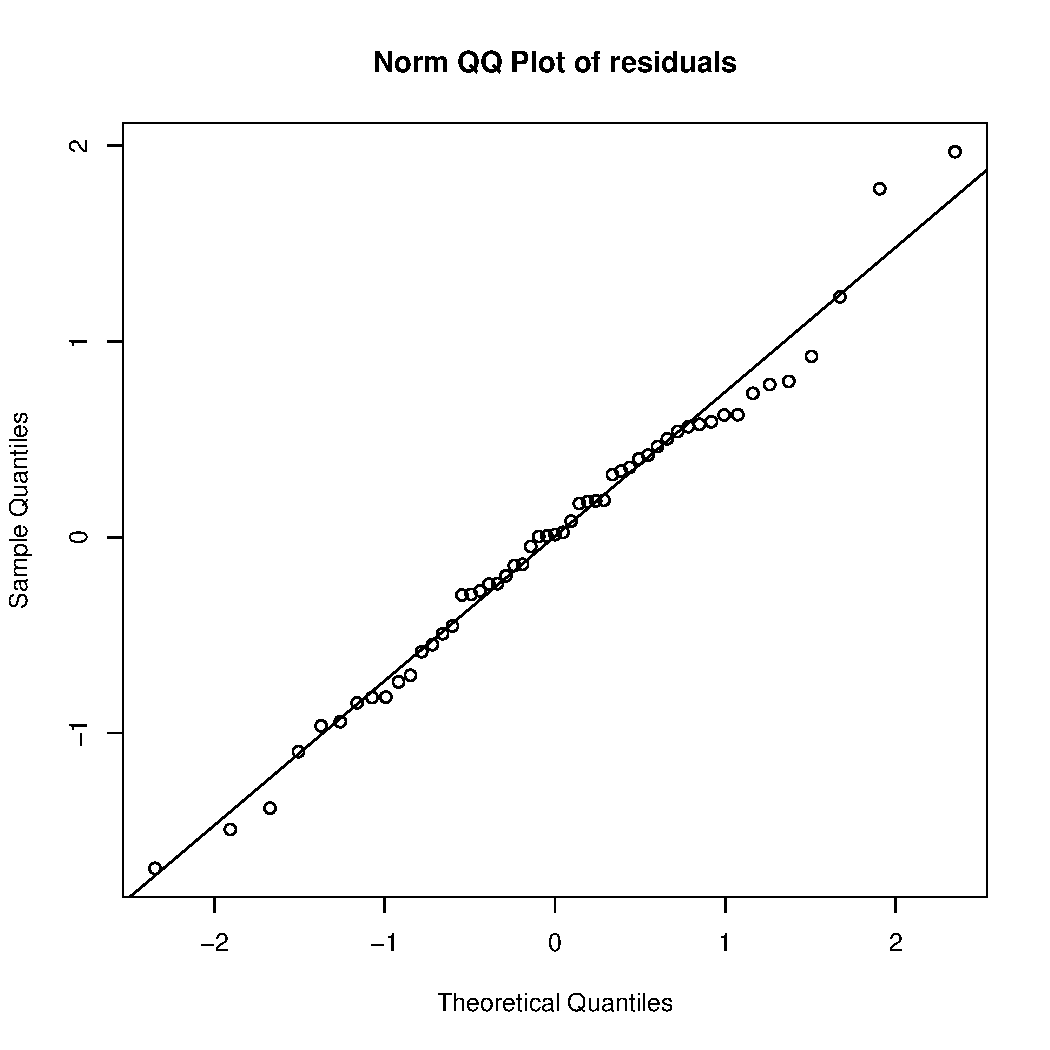
\includegraphics[scale =.4]{images/TEM22QQNorm.pdf}
    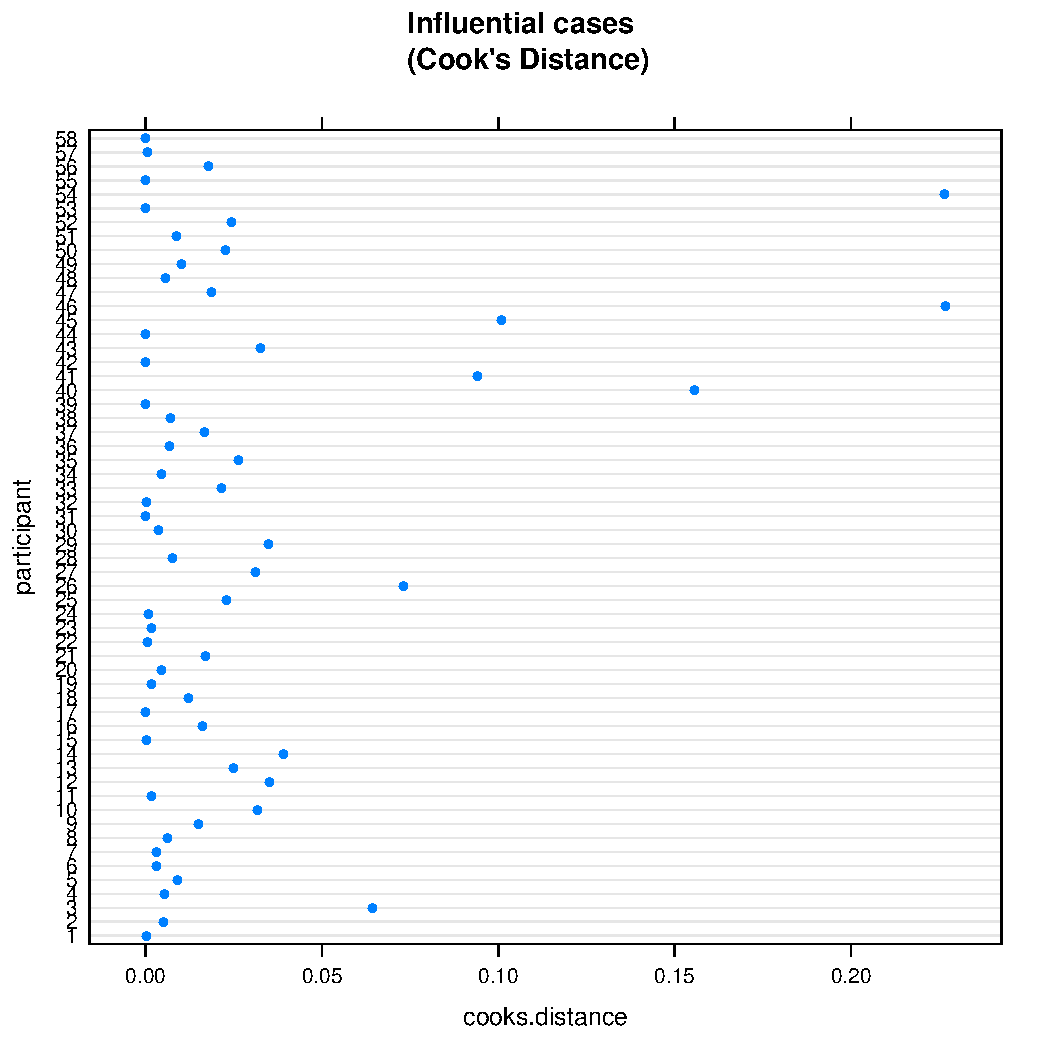
\includegraphics[scale =.4]{images/TEM22CooksD.pdf}
    \caption{Model 2.2 Assumptions: More positive change in perceptions of group performance predicts feelings of Social Bonding, moderated by condition}
    \label{fig:M22Assumptions}
\end{figure}

%M2.2
\begin{figure}[htbp]
    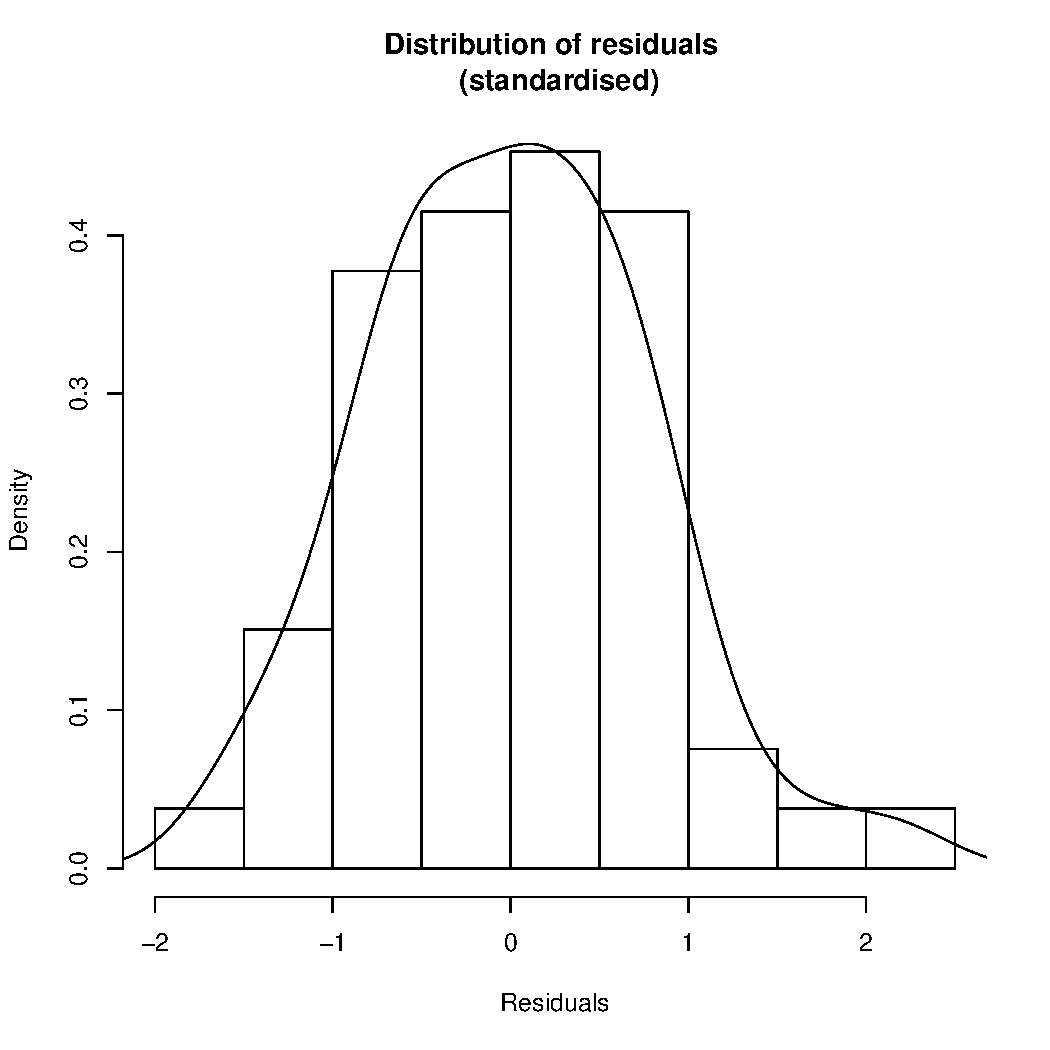
\includegraphics[scale =.4]{images/TEM23Hist.pdf}
    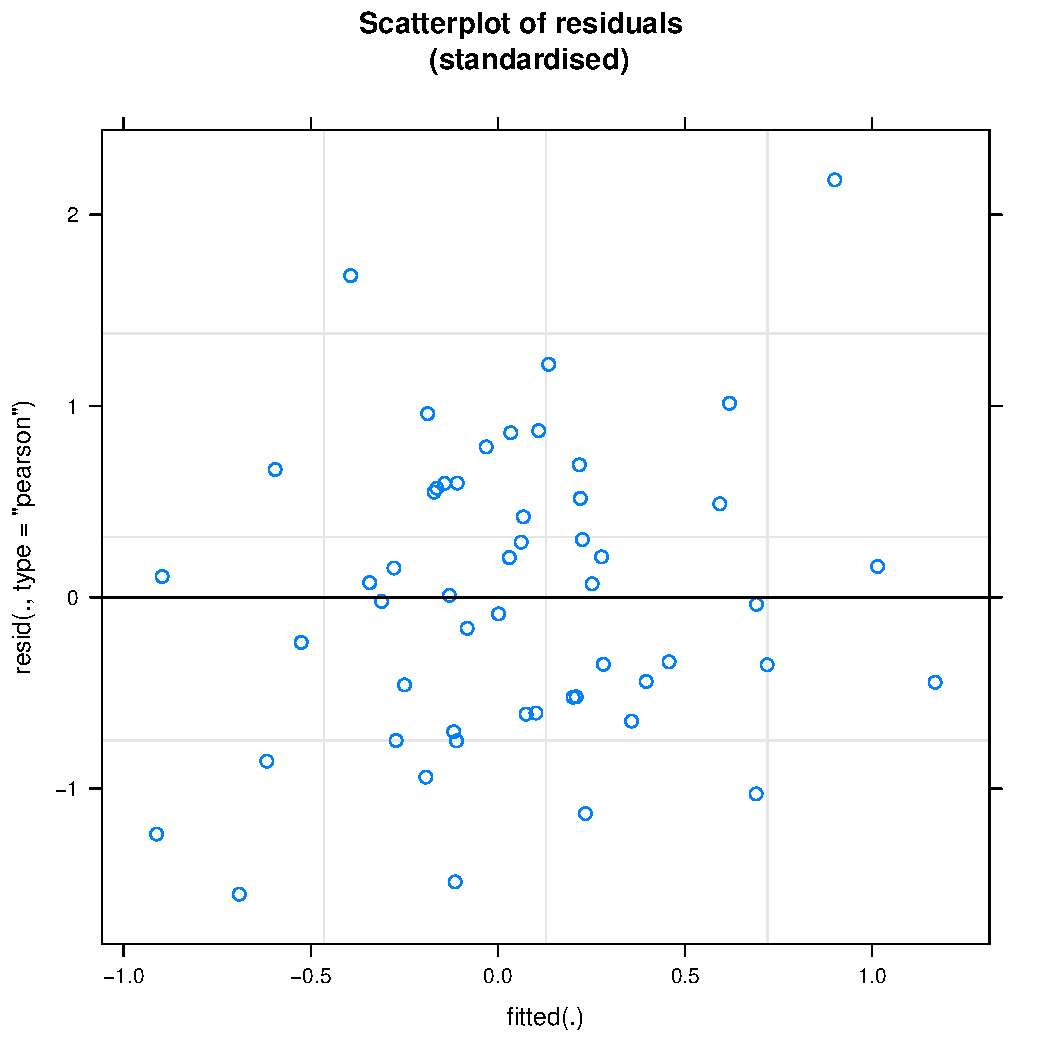
\includegraphics[scale =.4]{images/TEM23Scatter.pdf}
    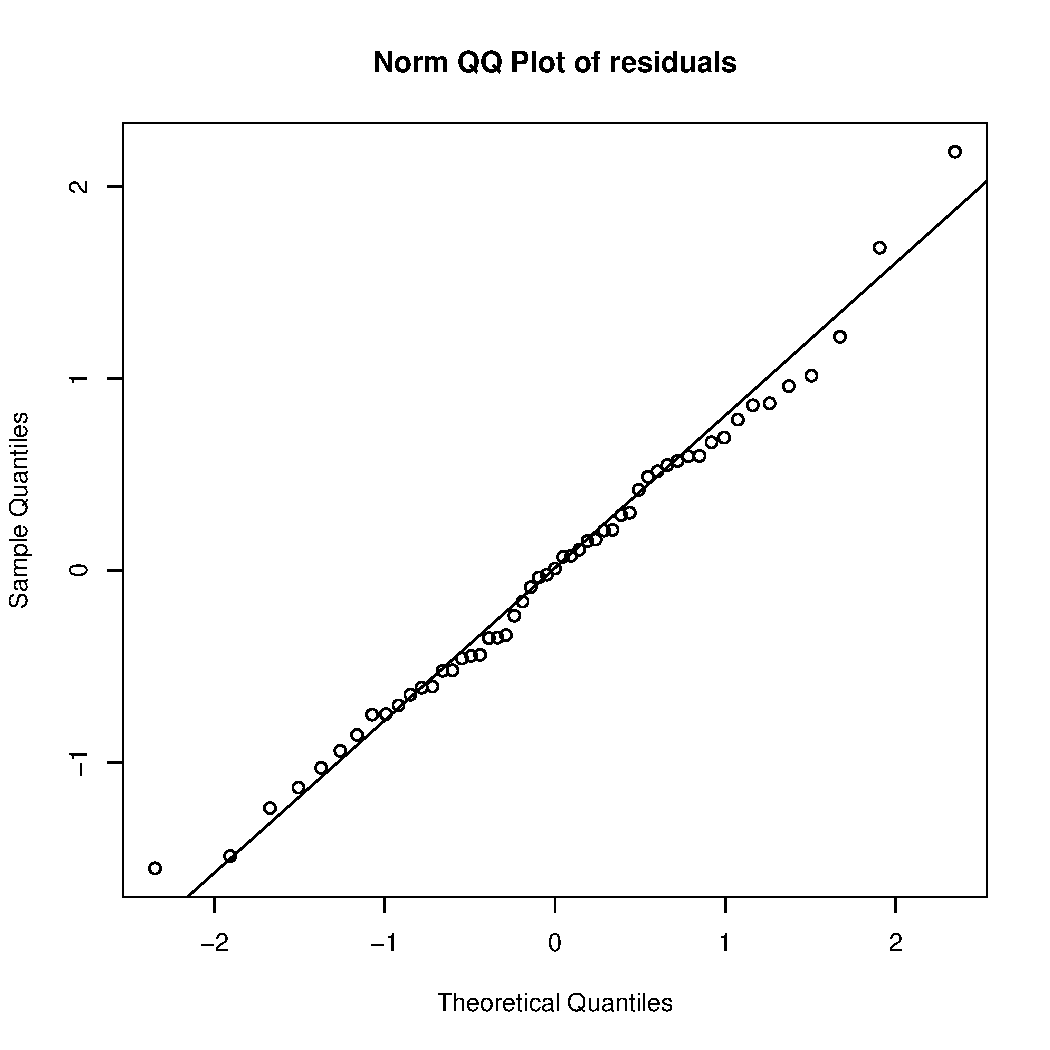
\includegraphics[scale =.4]{images/TEM23QQNorm.pdf}
    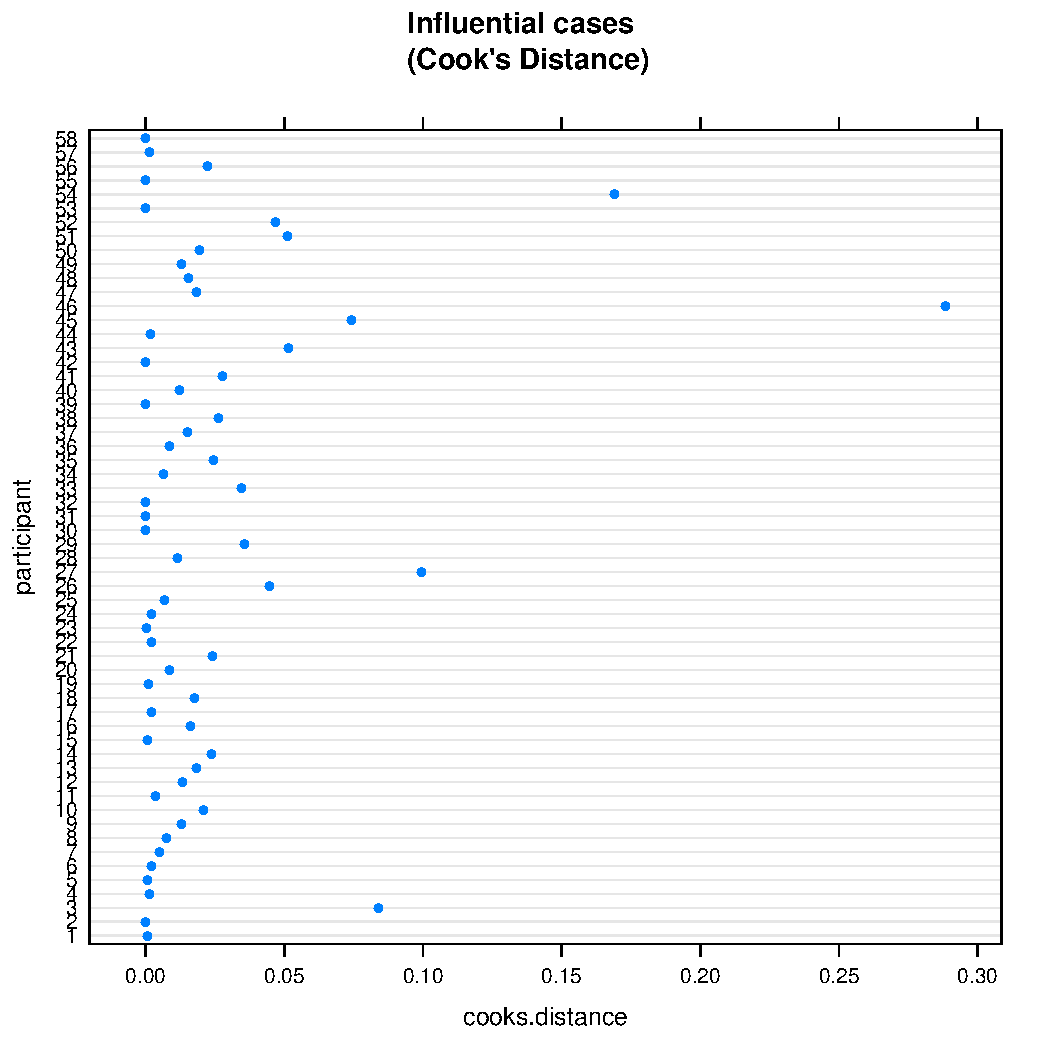
\includegraphics[scale =.4]{images/TEM23CooksD.pdf}
    \caption{Model 2.3 Assumptions: More positive change in perceptions of group performance predicts feelings of Social Bonding, moderated by condition}
    \label{fig:M23Assumptions}
\end{figure}













%%%%%%%%%%%%%%




Arousal post-Experiemnt:

\begin{figure}
  \centering
  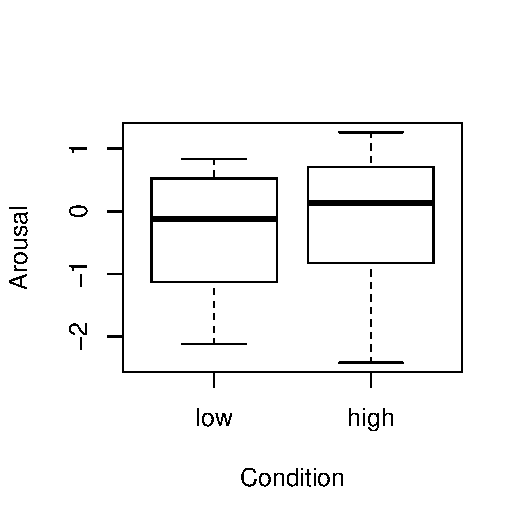
\includegraphics[width=0.5\linewidth,keepaspectratio] {images/arousalFactorPreBoxPlot-1}
  \caption{Athlete arousal prior to experiment, by condition}
        \label{fig:arousalFactorPreBoxPlot}
    \end{figure}

\begin{figure}
  \centering
      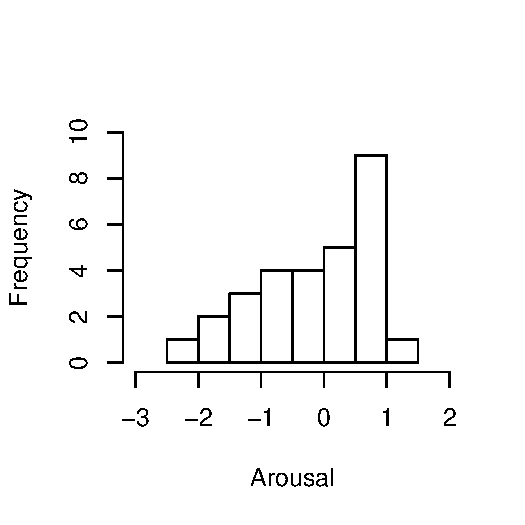
\includegraphics[width=0.5\linewidth,keepaspectratio] {images/histArousalFactorPreHigh-1}
      \caption{Histogram of athlete arousal prior to experiment (high difficulty condition)}
        \label{fig:histArousalFactorPreHigh}
    \end{figure}

\begin{figure}
  \centering
  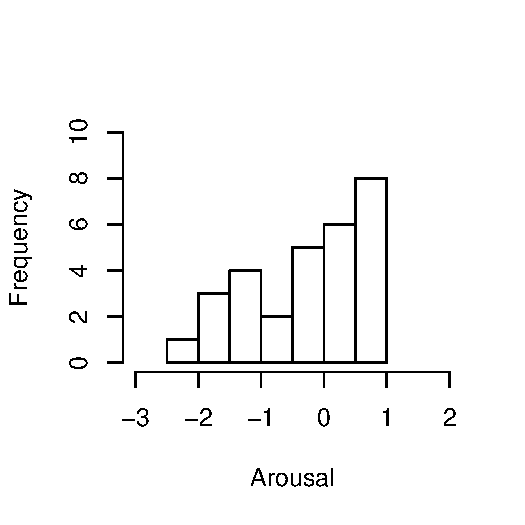
\includegraphics[width=0.5\linewidth,keepaspectratio] {images/histArousalFactorPreLow-1}
      \caption{Histogram of athlete arousal prior to experiment (low difficulty condition)}
  \caption{title}
    \label{fig:histArousalFactorPreLow}
\end{figure}














PRE-POST experiment results:

Histograms showing distribution of change variables:

"groupPerfChangeHist.pdf"
"indPerfChangeHist.pdf"
"groupClickChangeHist.pdf
"groupBondingChangeHist.pdf"
"teamBondingChangeHist.pdf"



Assumptions

~\ref{fig:M1PrePostAssumptions}


~\ref{fig:M2PrePostAssumptions}
